% ============================================================================
% Rapport de mini-projet : Santé digitale et ingénierie des systèmes de santé
% « SahaLink : plateforme de téléconsultation avec suivi à distance »
% Auteurs    : A. Issami, M. Ezbakhe, H. Benzahra, Z. Hsain, H. Kichchou, M. Hamdouch
% Encadrante : Prof. Maria Zemzami (ENSAM Rabat)
% ENSAM Rabat, filière INDIA&SD, année universitaire 2026/2027
% Compilation : make   (ou : pdflatex, bibtex, pdflatex, pdflatex)
% ============================================================================

\documentclass[11pt,a4paper,openany]{report}

% ============================================================================
% Préambule : rapport de mini-projet « SahaLink »
% ENSAM Rabat, filière INDIA&SD, Santé digitale, année universitaire 2026/2027
% Gabarit repris du rapport « Jumeau numérique d'une ligne de production »
% (même charte : bleu marine ENSAM, rouge du logo ENSAM).
% ============================================================================

\usepackage[utf8]{inputenc}
\usepackage[T1]{fontenc}
\usepackage[french]{babel}
\usepackage{lmodern}
\usepackage{geometry}
\usepackage{graphicx}
\usepackage{listings}
\usepackage{xcolor}
\usepackage{hyperref}
\usepackage{fancyhdr}
\usepackage{titlesec}
\usepackage{booktabs}
\usepackage{tabularx}
\usepackage{longtable}
\usepackage{enumitem}
\usepackage{tikz}
\usepackage{float}
\usepackage{amsmath}
\usepackage{amssymb}
\usepackage{caption}
\usepackage{subcaption}
\usepackage{tcolorbox}
\usepackage[nohyperlinks]{acronym}
\usepackage{csquotes}
\usepackage{colortbl}
\usepackage{multirow}
\usepackage{pgfplots}
\pgfplotsset{compat=1.18}

\usetikzlibrary{shapes.geometric, arrows.meta, positioning, fit, backgrounds, calc}

% ---------------------------- Mise en page ----------------------------------
\geometry{a4paper, margin=2.3cm, headheight=15pt}

\definecolor{ensambleu}{HTML}{1B3A5C}
\definecolor{ensamrouge}{HTML}{B22A2E}
\definecolor{lienviolet}{HTML}{4A148C}
\definecolor{vert}{HTML}{15803D}
\definecolor{orange}{HTML}{C2410C}

\hypersetup{
    colorlinks=true,
    linkcolor=lienviolet,
    urlcolor=lienviolet,
    citecolor=lienviolet,
    pdftitle={SahaLink : plateforme de téléconsultation avec suivi à distance},
    pdfauthor={Issami, Ezbakhe, Benzahra, Hsain, Kichchou, Hamdouch}
}

% ---------------------------- Listings (code) -------------------------------
\definecolor{codebg}{HTML}{F5F5F5}
\definecolor{codegreen}{HTML}{28A745}
\definecolor{codepurple}{HTML}{6F42C1}
\definecolor{codegray}{HTML}{6A737D}

\lstdefinestyle{mystyle}{
    backgroundcolor=\color{codebg},
    commentstyle=\color{codegray}\itshape,
    keywordstyle=\color{codepurple}\bfseries,
    numberstyle=\tiny\color{codegray},
    stringstyle=\color{codegreen},
    basicstyle=\ttfamily\footnotesize,
    breakatwhitespace=false,
    breaklines=true,
    captionpos=b,
    keepspaces=true,
    numbers=left,
    numbersep=5pt,
    showspaces=false,
    showstringspaces=false,
    showtabs=false,
    tabsize=2,
    frame=single,
    rulecolor=\color{gray!30},
    extendedchars=true,
    inputencoding=utf8,
    literate=%
      {é}{{\'e}}1 {è}{{\`e}}1 {ê}{{\^e}}1 {ë}{{\"e}}1
      {à}{{\`a}}1 {â}{{\^a}}1 {ä}{{\"a}}1
      {î}{{\^i}}1 {ï}{{\"i}}1
      {ô}{{\^o}}1 {ö}{{\"o}}1
      {ù}{{\`u}}1 {û}{{\^u}}1 {ü}{{\"u}}1
      {ç}{{\c c}}1 {Ç}{{\c C}}1
      {É}{{\'E}}1 {È}{{\`E}}1 {À}{{\`A}}1 {×}{{$\times$}}1 {·}{{\textperiodcentered}}1
}
\lstset{style=mystyle}

% ---------------------------- En-tête / pied --------------------------------
\renewcommand{\chaptermark}[1]{\markboth{\chaptername\ \thechapter}{}}

\pagestyle{fancy}
\fancyhf{}
\fancyhead[L]{\small\nouppercase{\leftmark}}
\fancyhead[R]{\small SahaLink, téléconsultation avec suivi à distance}
\fancyfoot[L]{\footnotesize ENSAM Rabat, Année Universitaire 2026/2027}
\fancyfoot[R]{\thepage}
\renewcommand{\headrulewidth}{0.4pt}
\renewcommand{\footrulewidth}{0.4pt}

\fancypagestyle{plain}{%
  \fancyhf{}%
  \fancyfoot[L]{\footnotesize ENSAM Rabat, Année Universitaire 2026/2027}%
  \fancyfoot[R]{\thepage}%
  \renewcommand{\headrulewidth}{0pt}%
  \renewcommand{\footrulewidth}{0.4pt}%
}

% ---------------------------- Titres chapitres ------------------------------
\titleformat{\chapter}[display]
  {\normalfont\huge\bfseries\color{ensambleu}}
  {\chaptertitlename\ \thechapter}{20pt}{\Huge}
\titlespacing*{\chapter}{0pt}{-20pt}{30pt}

% ---------------------------- Légendes --------------------------------------
\captionsetup{font=small, labelfont=bf, labelsep=period}

% ---------------------------- Macros utiles ---------------------------------
\newcommand{\code}[1]{\texttt{#1}}

\newtcolorbox{callout}[1][]{colback=ensambleu!5, colframe=ensambleu, sharp corners,
  boxrule=0.5pt, left=8pt, right=8pt, top=6pt, bottom=6pt, #1}
\newtcolorbox{success}[1][]{colback=green!6, colframe=green!60!black, sharp corners,
  boxrule=0.5pt, left=8pt, right=8pt, top=6pt, bottom=6pt, #1}
\newtcolorbox{warn}[1][]{colback=orange!6, colframe=orange!70!black, sharp corners,
  boxrule=0.5pt, left=8pt, right=8pt, top=6pt, bottom=6pt, #1}

% Introduction et conclusion de chapitre (sections non numérotées)
\newcommand{\introchap}{\section*{Introduction du chapitre}}
\newcommand{\conclchap}{\section*{Conclusion du chapitre}}

\setlist[itemize]{itemsep=2pt, topsep=3pt}
\setlist[enumerate]{itemsep=2pt, topsep=3pt}

% ---------------------------- Acronymes -------------------------------------
\acrodef{API}{Application Programming Interface}
\acrodef{ASGI}{Asynchronous Server Gateway Interface}
\acrodef{CNDP}{Commission nationale de contrôle de la protection des données à caractère personnel}
\acrodef{CSP}{Content Security Policy}
\acrodef{DTLS}{Datagram Transport Layer Security}
\acrodef{ENSAM}{École Nationale Supérieure d'Arts et Métiers}
\acrodef{HSTS}{HTTP Strict Transport Security}
\acrodef{HTTP}{HyperText Transfer Protocol}
\acrodef{HTTPS}{HyperText Transfer Protocol Secure}
\acrodef{ICE}{Interactive Connectivity Establishment}
\acrodef{INDIA}[INDIA\&SD]{Ingénierie Numérique en Data Science, Intelligence Artificielle \& Santé Digitale}
\acrodef{JSON}{JavaScript Object Notation}
\acrodef{NAT}{Network Address Translation}
\acrodef{OMS}{Organisation mondiale de la Santé}
\acrodef{PBKDF2}{Password-Based Key Derivation Function 2}
\acrodef{REST}{Representational State Transfer}
\acrodef{SDP}{Session Description Protocol}
\acrodef{SHA}{Secure Hash Algorithm}
\acrodef{SpO2}{Saturation pulsée en oxygène}
\acrodef{SQL}{Structured Query Language}
\acrodef{SRTP}{Secure Real-time Transport Protocol}
\acrodef{STUN}{Session Traversal Utilities for NAT}
\acrodef{SUS}{System Usability Scale}
\acrodef{TLS}{Transport Layer Security}
\acrodef{TURN}{Traversal Using Relays around NAT}
\acrodef{WS}{WebSocket}
\acrodef{XSS}{Cross-Site Scripting}

\endinput


\begin{document}

% ============================================================================
% Page de garde : deux logos, ENSAM (gauche) et Université Mohammed V (droite).
% ============================================================================

\begin{titlepage}
    \centering

    \begin{minipage}[c]{0.2\textwidth}
        \centering
        
\includegraphics[height=2.2cm]{images/logo_ensam.png}
    \end{minipage}\hfill
    \begin{minipage}[c]{0.56\textwidth}
        \centering
        {\normalsize\textbf{Université Mohammed V de Rabat}}\\[0.15cm]
        {\small École Nationale Supérieure d'Arts et Métiers}
    \end{minipage}\hfill
    \begin{minipage}[c]{0.2\textwidth}
        \centering
        
\includegraphics[height=2.2cm]{images/logo_um5.png}
    \end{minipage}\\[0.35cm]
    {\color{ensambleu}\rule{\textwidth}{0.8pt}}

    \vfill

    {\small F\,I\,L\,I\,È\,R\,E}\\[0.35cm]
    {\fontsize{50}{56}\selectfont\bfseries\textcolor{ensambleu}{INDIA\&SD}}\\[0.35cm]
    {\fontsize{20}{27}\selectfont\bfseries\textcolor{ensambleu}{Ingénierie Numérique en Data Science,\\ Intelligence Artificielle \& Santé Digitale}\par}

    \vfill

    {\color{ensambleu}\rule{\textwidth}{0.8pt}}\\[0.45cm]
    {\normalsize\bfseries R\,A\,P\,P\,O\,R\,T\quad D\,E\quad M\,I\,N\,I\,-\,P\,R\,O\,J\,E\,T}\\[0.15cm]
    {\small Santé digitale et ingénierie des systèmes de santé}\\[0.4cm]
    {\fontsize{24}{31}\selectfont\bfseries\textcolor{ensambleu}{SahaLink\\ Plateforme de téléconsultation\\ avec suivi à distance}\par}\vspace{0.4cm}
    {\normalsize Consultation vidéo WebRTC, suivi de constantes physiologiques\\[0.05cm]
     et alertes sur seuils, dans le cadre légal marocain}\\[0.35cm]
    {\color{ensambleu}\rule{\textwidth}{0.8pt}}\\[0.3cm]
    {\small\itshape Mini-projet n\textsuperscript{o}\,2 de la liste \enquote{Projets de santé digitale}}

    \vfill

    \begin{minipage}[t]{0.5\textwidth}
        \centering
        {\normalsize\textbf{Réalisé par}}\\[0.2cm]
        Aymane \textsc{Issami}\\[0.05cm]
        Marouan \textsc{Ezbakhe}\\[0.05cm]
        Hiba \textsc{Benzahra}\\[0.05cm]
        Zaid \textsc{Hsain}\\[0.05cm]
        Houssam \textsc{Kichchou}\\[0.05cm]
        Mohamed \textsc{Hamdouch}
    \end{minipage}\hfill
    \begin{minipage}[t]{0.46\textwidth}
        \centering
        {\normalsize\textbf{Encadré par}}\\[0.2cm]
        Prof. Maria \textsc{Zemzami} {\small (ENSAM)}
    \end{minipage}

    \vfill

    {\color{ensambleu}\rule{\textwidth}{0.8pt}}\\[0.2cm]
    {\small 3\textsuperscript{ème} année, S5, Année universitaire 2026/2027}

\end{titlepage}


\pagenumbering{roman}

\chapter*{Remerciements}
\addcontentsline{toc}{chapter}{Remerciements}
\markboth{Remerciements}{}

Au terme de ce mini-projet, nous tenons à remercier toutes les personnes qui ont contribué à sa réalisation.

Nos premiers remerciements s'adressent à \textbf{Prof.~Maria Zemzami}, qui a proposé et encadré ce projet dans le cadre du module \enquote{Santé digitale et ingénierie des systèmes de santé}. Son cahier des charges~\cite{zemzami2026} (objectifs, livrables, normes à respecter et grille d'évaluation) a structuré notre démarche du début à la fin, et ce rapport en reprend volontairement le plan.

Nous remercions également le corps professoral de l'\ac{ENSAM} de Rabat, et particulièrement les enseignants de la filière \ac{INDIA}, pour la qualité de la formation dispensée~: les compétences en programmation, en modélisation et en sécurité des systèmes d'information acquises au cours de notre cursus ont été mobilisées à chaque étape du projet.

Enfin, chaque membre de l'équipe remercie les cinq autres pour la rigueur et l'entraide dont chacun a fait preuve~: une plateforme de téléconsultation n'est utile que si l'interface du patient, celle du médecin, le serveur, la vidéo et la sécurité parlent le même langage, et cet accord s'est construit ensemble.

\vspace{2cm}
\begin{flushright}
\textit{A.~\textsc{Issami}, M.~\textsc{Ezbakhe}, H.~\textsc{Benzahra},}\\
\textit{Z.~\textsc{Hsain}, H.~\textsc{Kichchou}, M.~\textsc{Hamdouch}}\\
\textit{2026}
\end{flushright}

\clearpage
\chapter*{Résumé}
\addcontentsline{toc}{chapter}{Résumé}
\markboth{Résumé}{}

Ce rapport présente la conception et la réalisation de \textbf{SahaLink}, un prototype de plateforme de téléconsultation avec suivi à distance, développé dans le cadre du mini-projet~2 du module \enquote{Santé digitale et ingénierie des systèmes de santé} de l'\ac{ENSAM} Rabat. Le prototype relie un patient et un médecin~: le patient donne son consentement et saisit ses constantes physiologiques (tension, fréquence cardiaque, \ac{SpO2}, température), le médecin suit leur évolution sur des graphiques, reçoit en temps réel une alerte lorsqu'un seuil est dépassé, puis ouvre une consultation vidéo que le patient rejoint sur invitation.

Le système repose sur trois briques. Un \textbf{backend} FastAPI expose une \ac{API} \ac{REST} et deux canaux \ac{WS}~: l'un pour les alertes et les invitations, l'autre pour la signalisation \textbf{WebRTC}. Une \textbf{base SQLite} de sept tables conserve les patients, comptes, sessions, consentements, constantes, alertes et consultations. Une \textbf{interface web} en français propose un espace patient et un espace médecin. La vidéo circule directement entre les deux navigateurs, chiffrée de bout en bout, sans passer par le serveur.

La \textbf{sécurité} est traitée dans le code~: mots de passe hachés avec sel (\ac{PBKDF2}), jetons de session stockés sous forme d'empreinte, contrôle des rôles sur chaque route, consentement bloquant (HTTP~409), verrouillage après échecs de connexion, politique de sécurité du contenu, \ac{HTTPS} imposé et \ac{HSTS}. Le cadre légal (loi marocaine~09-08, loi~131-13, rapport de l'\ac{OMS}) a été lu dans les textes officiels et relié aux mesures du prototype.

La validation s'appuie sur \textbf{37 tests automatisés}, qui couvrent 92~\% du code du serveur, sur un scénario clinique complet incluant des cas dégradés, et sur des mesures chiffrées~: 6 profils dangereux détectés sur 6, 3 valeurs impossibles rejetées sur 3, écriture d'une mesure en 31~ms en médiane sur le serveur de test. Les limites, notamment des données entièrement simulées, l'absence de relais \ac{TURN} par défaut et de chiffrement des données au repos, sont discutées en conclusion.

\bigskip
\noindent\textbf{Mots-clés :} téléconsultation, télémédecine, suivi à distance, WebRTC, alertes sur seuils, FastAPI, SQLite, consentement, loi~09-08, loi~131-13.

\vspace{1cm}
\chapter*{Abstract}
\addcontentsline{toc}{chapter}{Abstract}
\markboth{Abstract}{}

This report presents the design and implementation of \textbf{SahaLink}, a teleconsultation and remote monitoring prototype built for the mini-project~2 of the \enquote{Digital health and health systems engineering} module at ENSAM Rabat. The patient gives consent and enters physiological readings (blood pressure, heart rate, oxygen saturation, temperature); the doctor follows them on charts, receives a real-time alert when a threshold is crossed, and starts a video consultation that the patient joins on invitation.

A FastAPI \textbf{backend} exposes a \ac{REST} \ac{API} and two WebSocket channels (alerts and invitations, WebRTC signalling). A seven-table \textbf{SQLite database} stores patients, accounts, sessions, consents, readings, alerts and consultations. A French \textbf{web interface} offers a patient space and a doctor space. Video flows directly between the two browsers, encrypted end to end, and never through the server.

\textbf{Security} is implemented in the code: salted password hashing, hashed session tokens, role checks on every route, a blocking consent gate, login lockout, a content security policy, enforced \ac{HTTPS} and \ac{HSTS}. The Moroccan laws~09-08 and~131-13 and the WHO telemedicine report were read in their official text and mapped to the prototype. Validation relies on \textbf{37 automated tests} covering 92\% of the server code, a complete clinical scenario with degraded cases, and measured results: 6 out of 6 dangerous profiles detected, 3 out of 3 impossible values rejected, a median write time of 31~ms on the test server. The limitations, including fully simulated data, no default TURN relay and no encryption at rest, are discussed in the conclusion.

\bigskip
\noindent\textbf{Keywords:} teleconsultation, telemedicine, remote monitoring, WebRTC, threshold alerts, FastAPI, SQLite, consent, Moroccan law~09-08.

\clearpage

\renewcommand{\contentsname}{Table des matières}
\setcounter{tocdepth}{1}
\tableofcontents
\clearpage
\listoffigures
\clearpage
\listoftables
\clearpage
\chapter*{Liste des acronymes}
\addcontentsline{toc}{chapter}{Liste des acronymes}
\markboth{Liste des acronymes}{}

\begin{acronym}[PBKDF2]
  \acro{API}{Application Programming Interface}
  \acro{ASGI}{Asynchronous Server Gateway Interface}
  \acro{CNDP}{Commission nationale de contrôle de la protection des données à caractère personnel}
  \acro{CSP}{Content Security Policy}
  \acro{DTLS}{Datagram Transport Layer Security}
  \acro{ENSAM}{École Nationale Supérieure d'Arts et Métiers}
  \acro{HSTS}{HTTP Strict Transport Security}
  \acro{HTTP}{HyperText Transfer Protocol}
  \acro{HTTPS}{HyperText Transfer Protocol Secure}
  \acro{ICE}{Interactive Connectivity Establishment}
  \acro{INDIA}[INDIA\&SD]{Ingénierie Numérique en Data Science, Intelligence Artificielle \& Santé Digitale}
  \acro{JSON}{JavaScript Object Notation}
  \acro{NAT}{Network Address Translation}
  \acro{OMS}{Organisation mondiale de la Santé}
  \acro{PBKDF2}{Password-Based Key Derivation Function 2}
  \acro{REST}{Representational State Transfer}
  \acro{SDP}{Session Description Protocol}
  \acro{SHA}{Secure Hash Algorithm}
  \acro{SpO2}{Saturation pulsée en oxygène}
  \acro{SQL}{Structured Query Language}
  \acro{SRTP}{Secure Real-time Transport Protocol}
  \acro{STUN}{Session Traversal Utilities for NAT}
  \acro{SUS}{System Usability Scale}
  \acro{TLS}{Transport Layer Security}
  \acro{TURN}{Traversal Using Relays around NAT}
  \acro{WS}{WebSocket}
  \acro{XSS}{Cross-Site Scripting}
\end{acronym}

\clearpage

\pagenumbering{arabic}
\setcounter{page}{1}

% ============================================================================
% Introduction générale
% ============================================================================
\chapter*{Introduction générale}
\addcontentsline{toc}{chapter}{Introduction générale}
\markboth{Introduction générale}{}

Entre deux visites physiques, l'état d'un patient suivi pour une maladie chronique peut se dégrader sans que personne ne le voie~: une tension qui monte, une saturation en oxygène qui baisse, une fièvre qui s'installe. Le patient n'a pas toujours de moyen simple de signaler une mesure anormale, et le médecin n'a pas de visibilité continue sur ses patients. La télémédecine propose de réduire ce délai de détection en combinant deux usages complémentaires~: le \textbf{suivi à distance} de constantes physiologiques, qui signale automatiquement les valeurs inquiétantes, et la \textbf{téléconsultation} vidéo, qui permet de réagir immédiatement.

Ce mini-projet, deuxième sujet de la liste proposée par Prof.~Maria Zemzami~\cite{zemzami2026}, demande de \textbf{développer une application permettant la consultation vidéo et le partage de constantes physiologiques suivies dans le temps, avec un système d'alerte sur des seuils}. Trois livrables sont attendus~: un prototype fonctionnel (front et back), un scénario complet patient-médecin, et une analyse des enjeux réglementaires (consentement, confidentialité). Trois références normatives s'imposent~: la technologie WebRTC, le rapport de l'Organisation mondiale de la Santé (\ac{OMS}) sur la télémédecine, et la loi marocaine~131-13 qui encadre la télémédecine. Le cadre général du module ajoute la loi~09-08 sur la protection des données personnelles.

Nous avons réalisé \textbf{SahaLink}, un prototype complet développé à six et versionné dans un dépôt Git~: un serveur FastAPI avec une base SQLite, une interface web en français pour le patient et pour le médecin, un système d'alertes en temps réel par \ac{WS}, et une visioconsultation WebRTC en pair à pair. Toutes les données sont fictives. La sécurité n'est pas un chapitre décoratif~: elle est implémentée dans le code, testée automatiquement et reliée article par article aux textes de loi que nous avons lus.

Le rapport suit le plan du cahier des charges. Le chapitre~\ref{chap:etat} présente brièvement l'état de l'art. Le chapitre~\ref{chap:cadrage} cadre le contexte de soins, les acteurs, les besoins et les spécifications. Le chapitre~\ref{chap:conception} expose la conception (architecture, modèle de données, parcours, protocole), et le chapitre~\ref{chap:realisation} sa réalisation. Le chapitre~\ref{chap:validation} documente la validation et les résultats chiffrés, y compris le nombre de tests. Le chapitre~\ref{chap:securite} traite de la sécurité, de la confidentialité et de la conformité réglementaire, et le chapitre~\ref{chap:organisation} des aspects organisationnels. Le chapitre~\ref{chap:conclusion} dresse le bilan, les limites assumées et les perspectives.

% ============================================================================
% Chapitre 1 : État de l'art (volontairement court)
% ============================================================================
\chapter{État de l'art}
\label{chap:etat}

\introchap

Ce chapitre rassemble, de façon volontairement brève, les notions sur lesquelles repose le projet~: la télémédecine telle que l'\ac{OMS} la définit, la technologie WebRTC pour la vidéo, le suivi à distance par seuils, et le cadre légal marocain. Il ne cherche pas l'exhaustivité~; il fixe le vocabulaire et justifie les choix des chapitres suivants.

\section{La télémédecine selon l'OMS}

L'\ac{OMS} a adopté une description large de la télémédecine~: la prestation de soins de santé, lorsque la distance est un facteur critique, par des professionnels de santé qui utilisent les technologies de l'information et de la communication pour échanger des informations utiles au diagnostic, au traitement et à la prévention, à la recherche et à l'évaluation, et à la formation continue~\cite{oms2010}. Le rapport précise quatre éléments communs à toute télémédecine~: elle vise à fournir un soutien clinique, elle cherche à surmonter les barrières géographiques, elle utilise différentes technologies de l'information et de la communication, et son but est d'améliorer les résultats de santé.

L'enquête mondiale de 2009 sur laquelle s'appuie le rapport a recueilli les réponses de 114 pays, soit 59~\% des États membres. Elle montre que la téléradiologie est le domaine le plus établi (33~\%), qu'environ 30~\% des pays ont une agence nationale de télémédecine, et que seuls 20~\% déclarent une évaluation publiée depuis 2006. Le coût perçu est l'obstacle le plus cité, tandis que les pays développés évoquent davantage les questions juridiques de vie privée et de confidentialité. Deux enseignements guident notre travail~: \textbf{évaluer} le système avec des mesures chiffrées, et \textbf{traiter explicitement la confidentialité}.

\section{Téléconsultation vidéo et WebRTC}

WebRTC est un ensemble de standards qui permet à deux navigateurs d'échanger de l'audio et de la vidéo directement, sans module externe~\cite{w3cwebrtc,rfc8825}. Le principe est de séparer trois fonctions~:

\begin{itemize}
  \item la \textbf{signalisation}, que l'application doit fournir elle-même (ici un canal \ac{WS}~\cite{rfc6455}) pour échanger les descriptions de session (\ac{SDP}) et les candidats de connexion~;
  \item la \textbf{traversée des réseaux}, par l'algorithme \ac{ICE}~\cite{rfc8445}, qui s'appuie sur un serveur \ac{STUN}~\cite{rfc8489} pour découvrir l'adresse publique de chaque navigateur et, si aucun chemin direct n'existe, sur un relais \ac{TURN}~\cite{rfc8656}~;
  \item le \textbf{transport sécurisé} des médias, chiffrés par \ac{DTLS} et \ac{SRTP}~\cite{rfc5764}.
\end{itemize}

L'avantage pour la télémédecine est double~: le flux vidéo ne transite pas par le serveur de l'application, qui ne peut donc ni le voir ni le stocker, et la charge serveur reste faible.

\section{Suivi à distance et alertes sur seuils}

Le suivi à distance consiste à faire mesurer des constantes (tension artérielle, fréquence cardiaque, \ac{SpO2}, température) au domicile du patient et à les transmettre au médecin. Pour ne pas submerger le médecin, un système d'alerte compare chaque mesure à des seuils et ne le prévient que lorsqu'une valeur sort de la plage acceptable. Les seuils de SahaLink sont des règles simples et explicites, inspirées de références médicales usuelles, qui servent à la démonstration~; ils ne sont pas validés cliniquement, et doivent l'être par un médecin avant tout usage réel.

\section{Cadre légal marocain}

Deux textes encadrent le projet. La loi~131-13 relative à l'exercice de la médecine~\cite{loi13113} consacre sa section~4 à la télémédecine (articles~99 à~102) et exige notamment le consentement exprès, libre et éclairé du patient. La loi~09-08~\cite{loi0908} protège les personnes physiques à l'égard du traitement de leurs données personnelles et range les données de santé parmi les données sensibles. Leur lecture détaillée et leur mise en œuvre font l'objet du chapitre~\ref{chap:securite}.

\section{Positionnement}

Une plateforme certifiée apporte une authentification forte, un hébergement agréé et une architecture multi-établissements. SahaLink, prototype à données fictives, démontre le parcours fonctionnel complet avec une vidéo en pair à pair chiffrée et aucune vidéo stockée, mais sans second facteur, sur un seul serveur et avec SQLite.

\conclchap

La télémédecine, telle que l'\ac{OMS} la décrit, associe un soutien clinique, la levée de la barrière de la distance, des technologies de l'information et un objectif de résultats de santé. WebRTC fournit une vidéo sécurisée sans passer par le serveur, et un système d'alertes sur seuils permet de n'alerter le médecin que lorsque c'est utile. Le cadre légal marocain impose le consentement et la protection des données de santé. Ces éléments fixent le cadre du chapitre suivant, qui précise le contexte de soins et les besoins que SahaLink doit satisfaire.

% ============================================================================
% Chapitre 2 : Cadrage et spécifications
% ============================================================================
\chapter{Cadrage et spécifications}
\label{chap:cadrage}

\introchap

Un prototype n'a de sens que s'il répond à un problème de soins précis. Ce chapitre situe SahaLink dans son contexte (établissement, service, acteurs, problème traité), formalise les besoins qu'il doit satisfaire, en fixe le périmètre, puis en déduit les spécifications fonctionnelles et techniques et les règles d'alerte retenues.

\section{Contexte de soins}

L'\textbf{établissement cible} est le service de cardiologie ou de médecine générale d'un centre de santé marocain qui suit des patients chroniques, notamment des patients hypertendus. Le \textbf{problème réel traité} est le suivant~: entre deux visites physiques, une dérive d'une constante physiologique (tension, \ac{SpO2}, fréquence cardiaque, température) peut passer inaperçue. Le patient n'a pas de moyen simple de signaler une mesure anormale, et le médecin n'a pas de visibilité continue. SahaLink raccourcit ce délai de détection et ouvre un canal de téléconsultation immédiat en cas d'alerte.

\section{Acteurs}

\begin{table}[H]
\centering
\caption{Acteurs du système.}
\label{tab:acteurs}
\begin{tabularx}{\textwidth}{@{}l l X@{}}
\toprule
\textbf{Acteur} & \textbf{Persona fictif} & \textbf{Rôle dans le parcours} \\
\midrule
Patient & Amal El Idrissi, 54 ans, hypertension & Donne ou refuse son consentement, saisit ses constantes, rejoint la consultation sur invitation \\
Médecin & Dr.~Benali & Suit ses patients, reçoit les alertes, les acquitte, démarre la consultation vidéo \\
Plateforme & SahaLink & Valide, enregistre, compare aux seuils, notifie, relaie la signalisation vidéo \\
\bottomrule
\end{tabularx}
\end{table}

Deux comptes de démonstration sont créés au premier démarrage (\code{dr.benali} et \code{amal}). Tout visiteur peut en outre créer son propre compte patient fictif~: le rôle est alors toujours \enquote{patient}, imposé par le serveur, et il n'existe qu'un seul compte médecin de démonstration.

\section{Besoins formalisés}

\begin{table}[H]
\centering
\caption{Besoins, réalisation dans SahaLink et vérification.}
\label{tab:besoins}
\small
\begin{tabularx}{\textwidth}{@{}l X X X@{}}
\toprule
\textbf{ID} & \textbf{Besoin} & \textbf{Réalisation} & \textbf{Vérification} \\
\midrule
B1 & S'identifier de façon sûre et ne voir que ce qui me concerne & Connexion, sessions, rôles & Tests de session et de droits \\
B2 & Donner ou refuser mon consentement & Consentement horodaté, démarrage bloqué sans accord & Test du refus HTTP~409 \\
B3 & Transmettre mes constantes depuis chez moi & Formulaire de saisie, historique personnel & Test de mesure normale \\
B4 & Être prévenu d'une constante anormale & Seuils, alerte en temps réel, acquittement & Tests d'alerte \\
B5 & Rejeter les valeurs impossibles & Bornes physiologiques côté serveur & Test HTTP~422 \\
B6 & Joindre rapidement le patient en vidéo & Invitation temps réel, code de salle aléatoire & Tests d'invitation \\
B7 & Rejoindre sans code technique & Bannière d'invitation, bouton \enquote{Rejoindre} & Test d'invitation \\
B8 & Que personne d'autre n'entre dans la consultation & Salle liée à un médecin et un patient, 2 participants au plus & Tests de signalisation \\
B9 & Retrouver une trace de l'acte & Table des consultations, données horodatées & Voir art.~100 (chapitre~\ref{chap:securite}) \\
B10 & Comprendre pourquoi la vidéo ne s'affiche pas & Choix de caméra, détection d'image noire & Test manuel \\
B11 & Créer mon propre compte patient & Inscription validée, rôle imposé, limitation de débit & Tests d'inscription \\
B12 & Suivre plusieurs patients et voir leur évolution & Liste des patients, quatre graphiques avec seuils & Tests de liste et de tableau de bord \\
\bottomrule
\end{tabularx}
\end{table}

\section{Périmètre}

\begin{table}[H]
\centering
\caption{Périmètre du projet.}
\label{tab:perimetre}
\begin{tabularx}{\textwidth}{@{}X X@{}}
\toprule
\textbf{Inclus} & \textbf{Exclu} \\
\midrule
Consentement, saisie et historique de constantes, alertes sur seuils en temps réel & Dispositifs de mesure connectés réels \\
Consultation vidéo WebRTC en pair à pair, invitation du patient & Enregistrement vidéo, partage d'écran, messagerie \\
Authentification, rôles, inscription patient & Vérification du statut de médecin, second facteur \\
Tableau de bord du médecin multi-patients avec graphiques & Gestion d'équipes soignantes, affectation d'un patient à un médecin \\
Données fictives et simulées documentées & Données de patients réels, hébergement agréé \\
\bottomrule
\end{tabularx}
\end{table}

\section{Spécifications fonctionnelles}

Le système doit permettre de créer un compte patient ou de se connecter avec un rôle~; de recueillir un consentement explicite (accepté ou refusé, avec finalité et date)~; d'enregistrer des constantes validées et de les afficher en tableau et en graphiques~; de comparer chaque mesure aux seuils et de transmettre l'alerte en temps réel au seul médecin~; de permettre au médecin d'acquitter l'alerte et de démarrer une consultation vidéo, refusée si le consentement manque~; et de permettre au patient de rejoindre puis de quitter la consultation, que le médecin termine.

\section{Spécifications techniques}

\subsection{Technologies retenues}

\begin{table}[H]
\centering
\caption{Choix technologiques.}
\label{tab:techno}
\begin{tabularx}{\textwidth}{@{}l l X@{}}
\toprule
\textbf{Couche} & \textbf{Technologie} & \textbf{Justification} \\
\midrule
Serveur & Python, FastAPI~\cite{fastapi}, Uvicorn & Routes \ac{REST} et \ac{WS} dans un seul outil, documentation automatique \\
Validation & Pydantic~\cite{pydantic} & Règles déclaratives, refus automatique (HTTP~422) \\
Base de données & SQLite~\cite{sqlite} & Aucune installation, démonstration reproductible \\
Temps réel & \ac{WS}~\cite{rfc6455} & Alertes et invitations sans interrogation périodique \\
Vidéo & WebRTC~\cite{w3cwebrtc} & Norme imposée, pair à pair, chiffrée \\
Interface & HTML, CSS, JavaScript & Aucune dépendance, graphiques en SVG intégré \\
\bottomrule
\end{tabularx}
\end{table}

Seules deux dépendances sont déclarées dans \code{requirements.txt} (FastAPI et Uvicorn)~: tout le reste provient de la bibliothèque standard de Python. Ce choix de sobriété rend l'installation immédiate et le code facile à expliquer.

\subsection{Règles d'alerte}

Les seuils, appliqués par le serveur à chaque mesure, sont des règles simples et déterministes.

\begin{table}[H]
\centering
\caption{Seuils d'alerte et bornes de validation.}
\label{tab:seuils}
\begin{tabular}{@{}lccc@{}}
\toprule
\textbf{Mesure} & \textbf{Alerte si} & \textbf{Gravité} & \textbf{Bornes acceptées} \\
\midrule
Tension & systolique $\geq 180$ ou diastolique $\geq 120$ mmHg & Critique & 70 à 250 / 40 à 160 \\
\ac{SpO2} & $< 90$~\% & Critique & 70 à 100~\% \\
Fréquence cardiaque & $< 45$ ou $> 130$ bpm & À surveiller & 30 à 220 bpm \\
Température & $\geq 39{,}0$~\textdegree C & À surveiller & 32 à 43~\textdegree C \\
\bottomrule
\end{tabular}
\end{table}

Plusieurs dépassements simultanés produisent \textbf{une seule alerte} qui les liste tous~; elle est critique dès qu'un des problèmes l'est. Il faut distinguer une valeur \textbf{impossible} (hors des bornes de validation, par exemple une tension de 500)~: elle est refusée et rien n'est enregistré~; et une valeur \textbf{dangereuse} (par exemple 188 de tension)~: elle est enregistrée et déclenche une alerte.

\subsection{Exigences non fonctionnelles}

\begin{itemize}
  \item \textbf{Confidentialité~:} aucune donnée n'est accessible sans session, et chaque rôle ne voit que ce qui le concerne.
  \item \textbf{Temps réel~:} une alerte ou une invitation doit parvenir sans rechargement de la page.
  \item \textbf{Reproductibilité~:} installation par une seule commande, tests rejouables sur une base temporaire.
  \item \textbf{Utilisabilité~:} interface en français, utilisable sur ordinateur et sur mobile.
  \item \textbf{Aucune donnée réelle~:} toutes les données sont fictives, conformément au cahier des charges.
\end{itemize}

\conclchap

Le cadrage fixe un problème de soins concret, trois acteurs, douze besoins reliés chacun à une vérification, un périmètre assumé et des règles d'alerte explicites. Les spécifications retenues privilégient la sobriété technique. Le chapitre suivant en déduit l'architecture, le modèle de données, le parcours patient-médecin et les protocoles d'échange.

% ============================================================================
% Chapitre 3 : Conception
% ============================================================================
\chapter{Conception de la plateforme}
\label{chap:conception}

\introchap

La conception transforme les besoins du chapitre précédent en une architecture, un modèle de données, un parcours et des protocoles d'échange. Ce chapitre présente successivement l'architecture générale, le modèle de données, le parcours patient-médecin modélisé en diagramme à couloirs, les protocoles (\ac{REST}, \ac{WS} et signalisation WebRTC), la matrice des droits par rôle, puis les principaux choix de conception et leur justification.

\section{Architecture générale}

Le système est découpé en trois couches (figure~\ref{fig:architecture})~: les \textbf{navigateurs} du patient et du médecin, le \textbf{serveur} FastAPI qui valide, enregistre et notifie, et la \textbf{base SQLite}. La vidéo n'est pas une quatrième couche~: elle circule directement entre les deux navigateurs.

\begin{figure}[H]
\centering
\begin{tikzpicture}[
  box/.style={draw=ensambleu, fill=ensambleu!6, rounded corners=3pt, minimum width=3.4cm, minimum height=1cm, align=center, font=\small},
  db/.style={draw=ensamrouge, fill=ensamrouge!6, rounded corners=3pt, minimum width=3.4cm, minimum height=1cm, align=center, font=\small},
  grp/.style={draw=gray!60, dashed, rounded corners=6pt, inner sep=8pt},
  arr/.style={-{Stealth[length=2.5mm]}, thick, ensambleu},
  lbl/.style={font=\scriptsize, fill=white, inner sep=1.5pt}
]
\node[box] (pat) {\textbf{Patient}\\ navigateur};
\node[box, below=1.3cm of pat] (doc) {\textbf{Médecin}\\ navigateur};
\node[grp, fit=(pat)(doc), label={[font=\small\bfseries]above:Navigateurs}] (nav) {};

\node[box, right=4.3cm of pat] (api) {\textbf{API REST}\\ \scriptsize constantes, consentements,\\ \scriptsize alertes, consultations};
\node[box, below=0.5cm of api] (ev) {\textbf{WebSocket /ws/events}\\ \scriptsize alertes, invitations};
\node[box, below=0.5cm of ev] (sig) {\textbf{WebSocket /ws/signaling}\\ \scriptsize relais \ac{SDP} et \ac{ICE}};
\node[grp, fit=(api)(ev)(sig), label={[font=\small\bfseries]above:Serveur FastAPI}] (srv) {};

\node[db, below=0.9cm of srv] (db) {\textbf{Base SQLite}\\ \scriptsize 7 tables};
\node[box, below=0.9cm of nav] (stun) {\textbf{\ac{STUN} / \ac{TURN}}\\ \scriptsize chemin réseau};

\draw[arr] (nav.east |- api) -- node[lbl, above]{REST + jeton} (api.west);
\draw[arr] (ev.west) -- node[lbl, above]{alertes, invitations} (nav.east |- ev);
\draw[arr, <->] (sig.west) -- node[lbl, above]{\ac{SDP}, \ac{ICE}} (nav.east |- sig);
\draw[arr] (srv.south) -- node[lbl, right]{SQL} (db.north);
\draw[arr, <->, ensamrouge, very thick] (pat.south) -- node[lbl, right]{vidéo et audio, \ac{DTLS}-\ac{SRTP}, pair à pair} (doc.north);
\draw[arr, dashed, gray] (stun.north) -- node[lbl, right]{candidats \ac{ICE}} (nav.south);
\end{tikzpicture}
\caption{Architecture de SahaLink.}
\label{fig:architecture}
\end{figure}

Le choix structurant est que \textbf{le serveur ne voit jamais l'image}. Il authentifie les deux participants, crée la consultation et relaie les messages de négociation, puis la vidéo s'établit directement entre les navigateurs. Le serveur ne stocke donc aucune vidéo, ce qui réduit à la fois la charge et l'exposition des données.

\section{Modèle de données}

La base compte sept tables (figure~\ref{fig:er}). Le \textbf{dernier consentement} d'un patient fait foi~: la téléconsultation ne peut démarrer que si cet enregistrement est une acceptation.

\begin{figure}[H]
\centering
\resizebox{\textwidth}{!}{%
\begin{tikzpicture}[
  ent/.style={draw=ensambleu, fill=ensambleu!5, rounded corners=2pt, align=left, font=\scriptsize, inner sep=4pt, minimum width=3.6cm},
  rel/.style={thick, ensambleu},
  lbl/.style={font=\tiny, fill=white, inner sep=1pt}
]
\node[ent] (consents) at (0,0) {\textbf{consents}\\ id (PK)\\ patient\_id (FK)\\ accepted\\ purpose\\ created\_at};
\node[ent] (patients) at (5.4,0) {\textbf{patients}\\ id (PK)\\ full\_name\\ birth\_year\\ care\_plan};
\node[ent] (vitals) at (10.8,0) {\textbf{vitals}\\ id (PK)\\ patient\_id (FK)\\ systolic, diastolic\\ heart\_rate, spo2\\ temperature\\ source, recorded\_at};
\node[ent] (users) at (0,-3.6) {\textbf{users}\\ id (PK)\\ username (unique)\\ display\_name\\ role\\ patient\_id (FK)\\ password\_salt, password\_hash};
\node[ent] (consult) at (5.4,-3.6) {\textbf{consultations}\\ id (PK)\\ room (unique)\\ doctor\_id (FK)\\ patient\_id (FK)\\ status\\ created\_at, ended\_at};
\node[ent] (alerts) at (10.8,-3.6) {\textbf{alerts}\\ id (PK)\\ patient\_id (FK)\\ vital\_id (FK)\\ severity, message\\ status, created\_at};
\node[ent] (sessions) at (0,-7.1) {\textbf{sessions}\\ token\_hash (PK)\\ user\_id (FK)\\ expires\_at};

\draw[rel] (patients) -- node[lbl, above]{1} (consents) node[lbl, above, pos=0.15]{N};
\draw[rel] (patients) -- node[lbl, above]{1} (vitals) node[lbl, above, pos=0.85]{N};
\draw[rel] (patients.south) -- node[lbl, right, pos=0.2]{1} node[lbl, right, pos=0.8]{N} (consult.north);
\draw[rel] (vitals.south) -- node[lbl, right, pos=0.2]{1} node[lbl, right, pos=0.8]{0..1} (alerts.north);
\draw[rel] (users.north east) -- node[lbl, above, pos=0.5]{0..1} (patients.south west);
\draw[rel] (users) -- node[lbl, above]{1} (consult) node[lbl, above, pos=0.85]{N};
\draw[rel] (users.south) -- node[lbl, right, pos=0.2]{1} node[lbl, right, pos=0.8]{N} (sessions.north);
\end{tikzpicture}}
\caption{Modèle entité-association (la table \code{alerts} référence aussi \code{patients} par \code{patient\_id}).}
\label{fig:er}
\end{figure}

Les sessions (\code{sessions}) ne conservent que l'empreinte du jeton et son expiration (8~h)~; les alertes (\code{alerts}) portent une gravité (\code{warning} ou \code{critical}) et un statut (\code{open} ou \code{acknowledged}).

\section{Parcours patient-médecin}

La figure~\ref{fig:bpmn} modélise le processus de bout en bout, avec un couloir par acteur, dans l'esprit de la notation BPMN. Elle couvre le parcours nominal et les cas dégradés, signalés en rouge.

\begin{figure}[H]
\centering
\resizebox{\textwidth}{!}{%
\begin{tikzpicture}[
  task/.style={draw=ensambleu, fill=white, rounded corners=3pt, minimum width=2.3cm, minimum height=1.3cm, align=center, font=\scriptsize, text width=2.15cm},
  lane/.style={draw=gray!50, fill=ensambleu!3},
  lname/.style={font=\footnotesize\bfseries, rotate=90, text=ensambleu},
  arr/.style={-{Stealth[length=2mm]}, thick, ensambleu},
  bad/.style={font=\scriptsize, text=ensamrouge, align=center}
]
\fill[lane] (-1.7,1.1) rectangle (18.4,-1.3);
\fill[lane, fill=ensamrouge!3] (-1.7,-1.3) rectangle (18.4,-3.9);
\fill[lane] (-1.7,-3.9) rectangle (18.4,-6.5);
\draw[gray!50] (-1.7,1.1) rectangle (18.4,-6.5);
\draw[gray!50] (-1.7,-1.3) -- (18.4,-1.3);
\draw[gray!50] (-1.7,-3.9) -- (18.4,-3.9);
\node[lname] at (-1.35,-0.1) {Patient};
\node[lname] at (-1.35,-2.6) {Système};
\node[lname] at (-1.35,-5.2) {Médecin};

\node[task] (p1) at (0,-0.1) {Créer un compte ou se connecter};
\node[task] (p2) at (2.8,-0.1) {Lire et accepter le consentement};
\node[task] (s1) at (2.8,-2.6) {Enregistrer le consentement};
\node[task] (p3) at (5.6,-0.1) {Saisir et envoyer une constante};
\node[task] (s2) at (8.4,-2.6) {Valider, enregistrer, comparer aux seuils, alerter};
\node[task] (d1) at (11.2,-5.2) {Recevoir l'alerte, consulter l'historique};
\node[task] (d2) at (14.0,-5.2) {Démarrer la consultation};
\node[task] (s5) at (14.0,-2.6) {Vérifier le consentement, créer la salle, inviter};
\node[task] (p5) at (14.0,-0.1) {Rejoindre la consultation vidéo};
\node[task] (d3) at (16.8,-5.2) {Terminer la consultation};

\draw[arr] (p1) -- (p2);
\draw[arr] (p2) -- (s1);
\draw[arr] (s1.east) -| (p3.south);
\draw[arr] (p3.east) -| (s2.north);
\draw[arr] (s2.east) -| (d1.north);
\draw[arr] (d1) -- (d2);
\draw[arr] (d2) -- (s5);
\draw[arr] (s5) -- (p5);
\draw[arr] (p5.east) -| (d3.north);

\node[bad] at (8.4,-3.6) {HTTP 422 si valeur impossible};
\node[bad, text width=2.2cm] at (15.7,-3.6) {HTTP 409 si accord absent ou retiré};
\node[bad] at (11.2,-6.2) {ou acquitter l'alerte, sans appel};
\end{tikzpicture}}
\caption{Parcours patient-médecin à trois couloirs, cas dégradés en rouge.}
\label{fig:bpmn}
\end{figure}

\section{Protocoles d'échange}

\subsection{Interface REST}

L'\ac{API} \ac{REST} regroupe quatre familles de routes~: les \textbf{comptes} (connexion, inscription, déconnexion), les \textbf{constantes et le consentement} d'un patient, les \textbf{alertes} (lecture et acquittement, réservés au médecin) et les \textbf{consultations} (démarrage, consultation active, fin). Le médecin dispose en plus de la liste des patients et du tableau de bord d'un patient. La liste complète des routes figure en annexe~\ref{ann:protocole}.

\subsection{Événements WebSocket}

Le canal \code{/ws/events} pousse des événements JSON vers les navigateurs authentifiés. Le médecin reçoit \code{alert}, \code{vital}, \code{consent} et \code{patient-registered}~; le patient reçoit \code{invitation} et \code{consultation-ended}. Un patient ne reçoit jamais les alertes du médecin.

\subsection{Signalisation WebRTC}

Le canal \code{/ws/signaling/\{room\}} ne fait que relayer les messages entre les deux participants. Après l'authentification (jeton dans le premier message), le serveur vérifie que l'utilisateur est bien le médecin ou le patient de la consultation ouverte, puis accepte au plus deux participants par salle. La figure~\ref{fig:sequence} montre l'enchaînement.

\begin{figure}[H]
\centering
\begin{tikzpicture}[
  life/.style={dashed, gray},
  actor/.style={draw=ensambleu, fill=ensambleu!8, rounded corners=2pt, minimum width=3cm, font=\small\bfseries, align=center},
  msg/.style={-{Stealth[length=2mm]}, thick, ensambleu},
  lbl/.style={font=\scriptsize, fill=white, inner sep=1pt}
]
\node[actor] (d) at (0,0) {Médecin\\ \scriptsize navigateur};
\node[actor] (s) at (5.5,0) {Serveur\\ \scriptsize signalisation};
\node[actor] (p) at (11,0) {Patient\\ \scriptsize navigateur};
\draw[life] (d.south) -- (0,-7.6);
\draw[life] (s.south) -- (5.5,-7.6);
\draw[life] (p.south) -- (11,-7.6);

\draw[msg] (0,-1.2) -- node[lbl, above]{auth (jeton)} (5.5,-1.2);
\draw[msg] (5.5,-1.7) -- node[lbl, above]{auth-ok} (0,-1.7);
\draw[msg] (11,-2.2) -- node[lbl, above]{auth (jeton)} (5.5,-2.2);
\draw[msg] (5.5,-2.7) -- node[lbl, above]{auth-ok} (11,-2.7);
\draw[msg] (0,-3.4) -- node[lbl, above]{offre (\ac{SDP})} (5.5,-3.4);
\draw[msg] (5.5,-3.6) -- node[lbl, above]{relais} (11,-3.6);
\draw[msg] (11,-4.3) -- node[lbl, above]{réponse (\ac{SDP})} (5.5,-4.3);
\draw[msg] (5.5,-4.5) -- node[lbl, above]{relais} (0,-4.5);
\draw[msg, <->] (0,-5.2) -- node[lbl, above]{candidats \ac{ICE}} (5.5,-5.2);
\draw[msg, <->] (5.5,-5.4) -- node[lbl, above]{candidats \ac{ICE}} (11,-5.4);
\draw[msg, <->, ensamrouge, very thick] (0,-6.6) -- node[lbl, above]{média direct, chiffré \ac{DTLS}-\ac{SRTP}} (11,-6.6);
\end{tikzpicture}
\caption{Établissement de la vidéo~: le serveur ne relaie que la négociation.}
\label{fig:sequence}
\end{figure}

\section{Droits par rôle}

\begin{table}[H]
\centering
\caption{Droits par rôle (appliqués par le serveur sur chaque route).}
\label{tab:droits}
\begin{tabular}{@{}p{5.4cm} >{\centering\arraybackslash}p{4.7cm} >{\centering\arraybackslash}p{4.7cm}@{}}
\toprule
\textbf{Action} & \textbf{Médecin} & \textbf{Patient} \\
\midrule
Se connecter, consulter sa session & oui & oui \\
Créer un compte & non & oui (rôle imposé) \\
Lire les constantes d'un dossier & oui & uniquement le sien \\
Envoyer une constante & oui & uniquement pour lui \\
Donner ou retirer le consentement & non (403) & uniquement pour lui \\
Lister les patients, lire alertes et tableau de bord & oui & non (403) \\
Acquitter une alerte & oui & non (403) \\
Démarrer une téléconsultation & oui, si consentement (sinon 409) & non (403) \\
Rejoindre la salle vidéo & si c'est sa consultation & si c'est sa consultation \\
Terminer la consultation & oui & non (il peut quitter et revenir) \\
\bottomrule
\end{tabular}
\end{table}

\section{Choix de conception et justification}

\begin{itemize}
  \item \textbf{WebRTC en pair à pair}~: norme imposée par le sujet~; le flux ne passe pas par le serveur, qui ne stocke aucune vidéo.
  \item \textbf{\ac{REST} pour les données, \ac{WS} pour le temps réel}~: une alerte ou une invitation doit arriver sans interrogation périodique.
  \item \textbf{Authentification dans le premier message \ac{WS}}~: le jeton n'apparaît jamais dans l'adresse, donc ni dans les journaux ni dans l'historique du navigateur~; l'origine de la page est vérifiée contre le détournement de WebSocket.
  \item \textbf{Code de salle aléatoire lié à un médecin et un patient}~: une salle ne peut être ni devinée ni rejointe par un tiers.
  \item \textbf{Pairs \enquote{polis}}~: si les deux navigateurs envoient une offre en même temps, l'un cède, ce qui évite les appels bloqués.
  \item \textbf{Choix de la caméra}~: les caméras virtuelles de téléphone sont classées en dernier et chaque caméra est testée sur une image réelle avant usage.
  \item \textbf{SQLite}~: aucune installation, démonstration reproductible~; l'accès passe par une seule fonction de connexion, ce qui faciliterait une migration vers PostgreSQL.
  \item \textbf{Seuils simples et explicites}, et \textbf{validation Pydantic} avant toute écriture en base.
\end{itemize}

\conclchap

L'architecture sépare nettement les rôles~: le navigateur présente, le serveur valide, enregistre et notifie, la base conserve, et la vidéo circule directement entre les pairs. Le modèle de données de sept tables, le parcours à trois couloirs et les protocoles forment le contrat sur lequel s'appuie la réalisation décrite au chapitre suivant.

% ============================================================================
% Chapitre 4 : Réalisation
% ============================================================================
\chapter{Réalisation du prototype}
\label{chap:realisation}

\introchap

Ce chapitre décrit comment la conception a été réalisée. Il présente l'organisation du dépôt, le serveur et ses routes, la base de données et l'authentification, les canaux temps réel, les interfaces du patient et du médecin, la visioconsultation côté navigateur, puis l'installation et le déploiement. Les extraits de code sont ceux du dépôt.

\section{Organisation du dépôt}

\begin{lstlisting}[language={}, numbers=none, caption={Arborescence du dépôt.}]
app/       main.py       FastAPI : routes REST, WebSocket, sécurité
           auth.py       connexion, sessions, jetons
           database.py   schéma SQLite, hachage des mots de passe
static/    index.html, styles.css
           app.js        interfaces patient et médecin, graphiques, WebRTC
tests/     test_api.py   37 tests automatisés
scripts/   benchmark.py  mesures chiffrées
           smoke_test.py parcours complet contre n'importe quelle adresse
           sus_score.py  calcul du score d'utilisabilité
docs/      architecture, BPMN, sécurité, validation, rapport/
\end{lstlisting}

L'application se lance par une seule commande (\code{uvicorn app.main:app}) et s'ouvre à l'adresse \code{http://127.0.0.1:8000}. Le serveur sert aussi les fichiers de l'interface~: aucun serveur web séparé n'est nécessaire.

\section{Le serveur FastAPI}

\subsection{Validation des données}

Les règles de validation sont déclarées une seule fois, dans des classes Pydantic. Une valeur hors bornes est refusée par le framework avec le code HTTP~422, avant même d'atteindre la base.

\begin{lstlisting}[language=Python, caption={Validation d'une mesure (extrait de \code{app/main.py}).}, label=lst:validation]
class VitalInput(BaseModel):
    systolic: int = Field(ge=70, le=250)
    diastolic: int = Field(ge=40, le=160)
    heart_rate: int = Field(ge=30, le=220)
    spo2: int = Field(ge=70, le=100)
    temperature: float = Field(ge=32, le=43)
\end{lstlisting}

\subsection{Règles d'alerte}

La fonction \code{alert\_for} compare une mesure validée aux seuils du tableau~\ref{tab:seuils}. Elle retourne au plus une alerte, qui regroupe tous les dépassements et dont la gravité est critique dès qu'un problème l'est.

\begin{lstlisting}[language=Python, caption={Règles d'alerte (\code{alert\_for}).}, label=lst:alert]
def alert_for(vital: VitalInput):
    issues = []
    if vital.systolic >= 180 or vital.diastolic >= 120:
        issues.append("Tension artérielle critique")
    if vital.spo2 < 90:
        issues.append("Saturation en oxygène critique")
    if vital.heart_rate < 45 or vital.heart_rate > 130:
        issues.append("Fréquence cardiaque hors seuil")
    if vital.temperature >= 39.0:
        issues.append("Fièvre élevée")
    if not issues:
        return None
    severity = "critical" if any("critique" in i for i in issues) else "warning"
    return severity, " · ".join(issues)
\end{lstlisting}

\subsection{Contrôle d'accès}

Chaque route appelle l'une de trois petites fonctions. L'interface masque certains menus pour le confort, mais c'est le serveur qui décide réellement.

\begin{lstlisting}[language=Python, caption={Contrôle de la session et des rôles.}, label=lst:roles]
def current_user(request: Request) -> dict:
    user = user_for_token(bearer_token(request))
    if not user:
        raise HTTPException(401, "Session absente ou expirée. Veuillez vous reconnecter.")
    return user

def doctor_only(user: dict = Depends(current_user)) -> dict:
    if user["role"] != "doctor":
        raise HTTPException(403, "Action réservée au médecin.")
    return user

def ensure_patient_access(user: dict, patient_id: int) -> None:
    if user["role"] == "patient" and user["patient_id"] != patient_id:
        raise HTTPException(403, "Accès refusé à ce dossier patient.")
\end{lstlisting}

\subsection{Envoi d'une mesure}

La route d'envoi d'une mesure enchaîne vérification des droits, validation, enregistrement et comparaison aux seuils. Selon le résultat, le médecin reçoit un événement \code{alert} ou un événement \code{vital}, de façon asynchrone, sans retarder la réponse au patient.

\section{Base de données et authentification}

La base est un fichier SQLite accédé par une seule fonction de connexion, qui ouvre, valide puis ferme. Les requêtes sont toutes paramétrées, ce qui rend l'injection \ac{SQL} impossible. Les mots de passe ne sont jamais conservés en clair~: ils sont transformés par \ac{PBKDF2} avec \ac{SHA}-256, 200\,000 itérations et un sel aléatoire propre à chaque compte~\cite{rfc8018}.

\begin{lstlisting}[language=Python, caption={Hachage et vérification des mots de passe (\code{app/database.py}).}, label=lst:hash]
PBKDF2_ITERATIONS = 200_000

def hash_password(password: str, salt_hex: str):
    return hashlib.pbkdf2_hmac(
        "sha256", password.encode(), bytes.fromhex(salt_hex), PBKDF2_ITERATIONS
    ).hex()

def verify_password(password: str, salt_hex: str, expected_hex: str) -> bool:
    return hmac.compare_digest(hash_password(password, salt_hex), expected_hex)
\end{lstlisting}

À la connexion, le serveur génère un jeton aléatoire de 32~octets et ne conserve en base que son empreinte \ac{SHA}-256, avec une validité de 8~heures. Une fuite de la base ne donne donc aucune connexion exploitable. Comme le hachage est volontairement lent, il s'exécute dans un fil séparé pour ne pas bloquer les autres requêtes.

\section{Canaux temps réel}

Deux \ac{WS} sont ouverts par le navigateur. Le premier message de chaque connexion doit être \code{\{"type": "auth", "token": ...\}}~: sans jeton valide, le serveur répond \code{auth-failed} et ferme la connexion. L'origine de la page est contrôlée, y compris derrière un proxy, pour bloquer le détournement de WebSocket depuis un autre site. La signalisation vérifie en plus que l'utilisateur est le médecin ou le patient de la consultation ouverte (sinon \code{forbidden}) et limite la salle à deux participants (sinon \code{room-full}). Quand l'un des deux quitte la salle, l'autre reçoit un message \code{leave} et peut attendre son retour.

\section{Interfaces utilisateur}

L'interface est en français et fonctionne sur ordinateur et sur mobile. Elle propose un écran de connexion avec deux comptes de démonstration, un formulaire d'inscription validé côté client et côté serveur, un espace patient et un espace médecin.

\begin{figure}[htbp]
\centering
\begin{subfigure}[t]{0.38\textwidth}
  \centering
  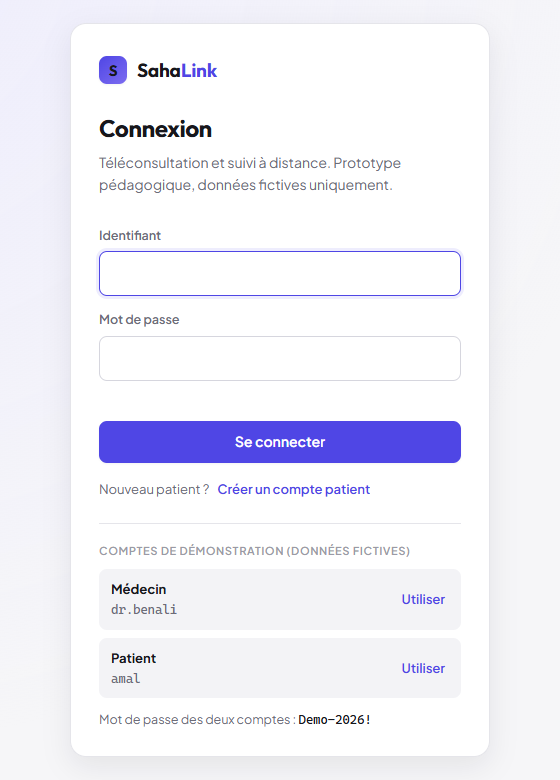
\includegraphics[width=\textwidth]{images/screenshots/connexion_crop.png}
  \caption{Connexion.}
\end{subfigure}\hfill
\begin{subfigure}[t]{0.38\textwidth}
  \centering
  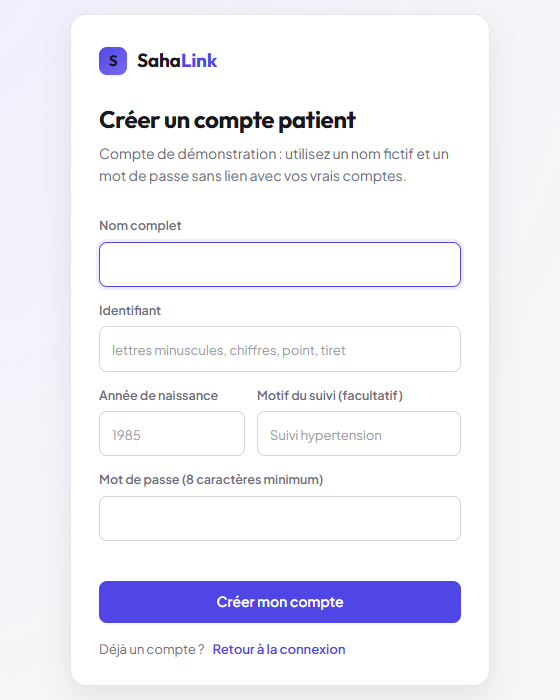
\includegraphics[width=\textwidth]{images/screenshots/inscription_crop.png}
  \caption{Inscription d'un patient.}
\end{subfigure}
\caption{Écrans d'accès (données fictives).}
\label{fig:acces}
\end{figure}

\subsection{Espace patient}

Le patient donne ou retire son consentement (case à cocher et bouton), saisit ses cinq constantes, peut préremplir des valeurs dangereuses avec le bouton \enquote{Simuler une alerte} (utile à la démonstration), consulte son historique et rejoint la consultation lorsqu'il est invité.

\begin{figure}[htbp]
\centering
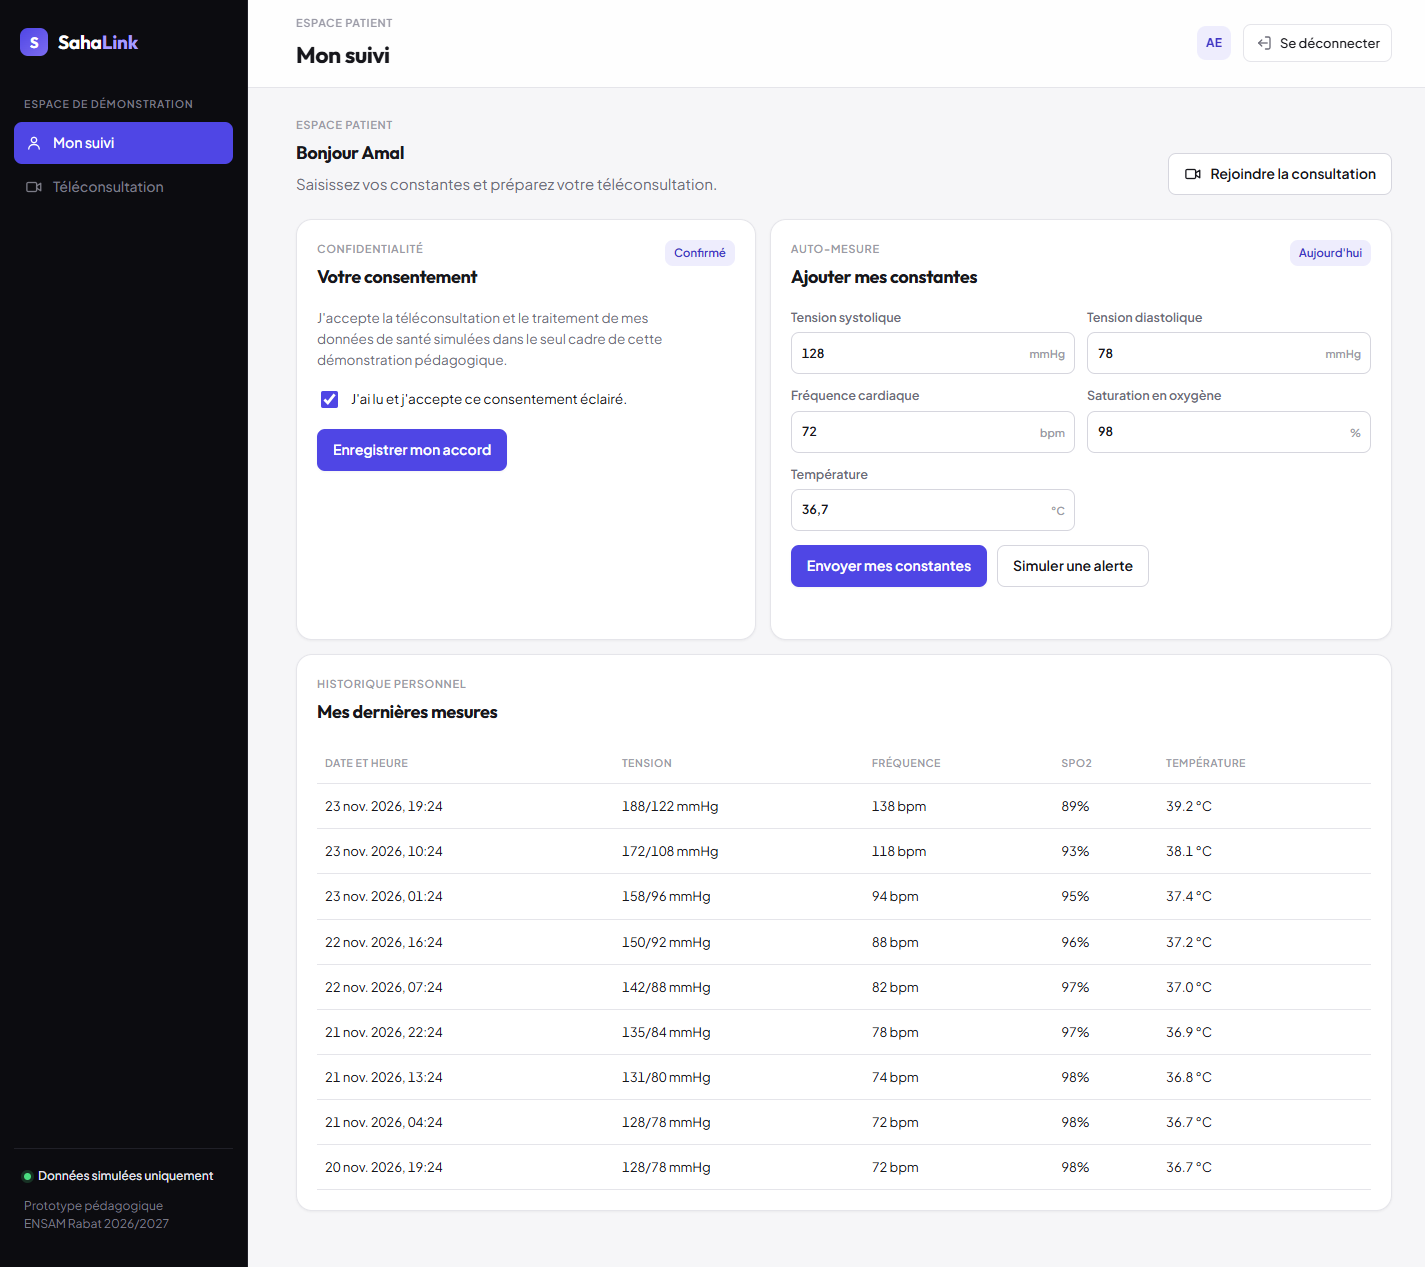
\includegraphics[width=0.46\textwidth]{images/screenshots/patient.png}
\caption{Espace patient~: consentement, saisie des constantes et historique personnel.}
\label{fig:patient}
\end{figure}

\subsection{Espace médecin}

Le médecin voit le nombre de patients suivis et d'alertes ouvertes, choisit un patient dans une liste qui indique pour chacun les alertes ouvertes et l'état du consentement, lit les valeurs courantes, reçoit les alertes en temps réel et peut les acquitter. Quatre petits graphiques en SVG intégré (tension, fréquence cardiaque, \ac{SpO2}, température) montrent l'évolution des mesures avec des lignes de seuil~: les points rouges signalent une valeur critique et les points orange une valeur à surveiller.

\begin{figure}[htbp]
\centering
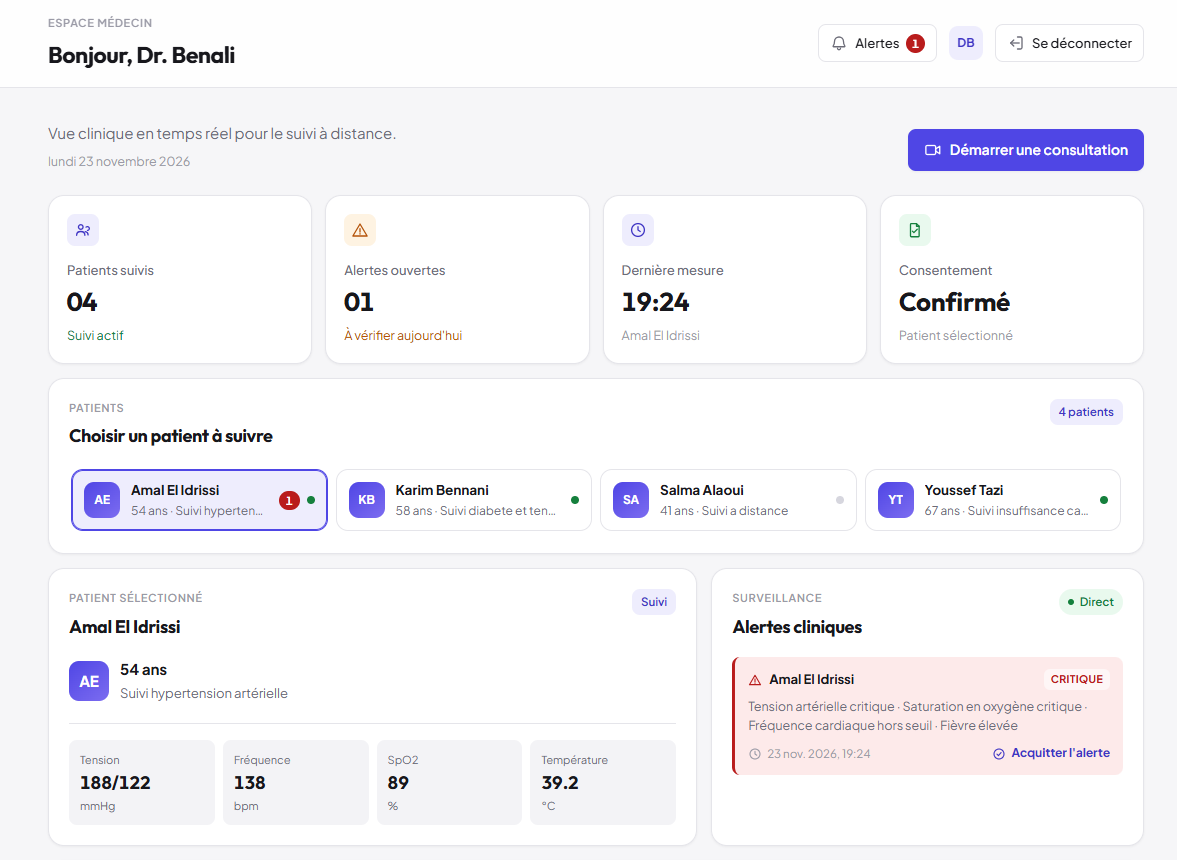
\includegraphics[width=0.74\textwidth]{images/screenshots/medecin_haut.png}
\caption{Espace médecin~: liste des patients, alerte critique et valeurs courantes (données fictives).}
\label{fig:medecin}
\end{figure}

\begin{figure}[htbp]
\centering
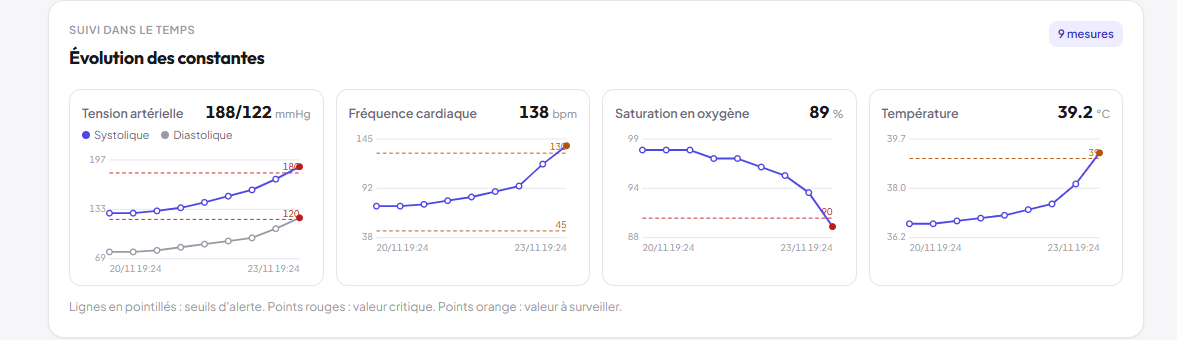
\includegraphics[width=0.74\textwidth]{images/screenshots/medecin_graphiques.png}
\caption{Évolution des quatre constantes avec lignes de seuil (pointillés) et points d'alerte.}
\label{fig:graphiques}
\end{figure}

\section{Visioconsultation côté navigateur}

La vidéo est gérée par le code JavaScript de \code{static/app.js}, qui crée une connexion \code{RTCPeerConnection} par appel. Quatre points méritent d'être signalés.

\begin{itemize}
  \item \textbf{Négociation sans blocage}~: le code applique le motif des pairs \enquote{polis}. Si les deux navigateurs envoient une offre en même temps, l'un abandonne la sienne pour accepter celle de l'autre.
  \item \textbf{Choix de la caméra}~: les caméras virtuelles de téléphone (Camo, Iriun) sont classées en dernier, et chaque candidate est testée sur une image réelle (mesure de la luminosité) avant d'être retenue. Une liste permet de changer de caméra en cours d'appel sans renégocier.
  \item \textbf{Diagnostic explicite}~: si la caméra renvoie une image noire, le statut dit si le problème vient de la caméra locale ou de celle de l'interlocuteur.
  \item \textbf{Serveurs de traversée}~: la configuration \ac{ICE} est servie par la route \code{/api/rtc-config}. Par défaut, des serveurs \ac{STUN} publics sont utilisés~; un relais \ac{TURN} peut être ajouté par la variable d'environnement \code{ICE\_SERVERS} pour les réseaux stricts.
\end{itemize}

La capture réelle de la caméra et du micro ne peut pas être automatisée~: elle est validée manuellement sur deux navigateurs (chapitre~\ref{chap:validation}).

\section{Installation et déploiement}

Trois variables d'environnement règlent le comportement~: \code{SAHALINK\_DB\_PATH} (fichier SQLite, utilisé par les tests pour une base temporaire), \code{ICE\_SERVERS} (liste \ac{JSON} de serveurs \ac{STUN} ou \ac{TURN}) et \code{SAHALINK\_FORCE\_HTTPS} (redirection vers HTTPS). Pour une démonstration entre deux ordinateurs, la caméra exige un contexte sécurisé~: le serveur local est exposé par un tunnel \ac{HTTPS} (Cloudflare), qui fournit aussi le chiffrement du transport. Un \code{Procfile} et un plan de déploiement sont fournis pour un hébergement qui accepte un serveur de longue durée (les \ac{WS} excluent les plateformes sans serveur). La procédure complète figure en annexe~\ref{ann:installation}.

\conclchap

La réalisation tient en trois fichiers Python et un fichier JavaScript. Les règles du chapitre~\ref{chap:cadrage} sont déclarées une seule fois (Pydantic, \code{alert\_for}, fonctions de contrôle), la sécurité des secrets est intégrée au schéma (sel, empreinte du jeton), et les deux interfaces affichent les mêmes données avec des droits différents. Le chapitre suivant évalue ce prototype par un scénario clinique complet, des tests automatiques et des mesures chiffrées.

% ============================================================================
% Chapitre 5 : Validation et résultats
% ============================================================================
\chapter{Validation et résultats}
\label{chap:validation}

\introchap

Un prototype n'est crédible que s'il est évalué. Ce chapitre présente le protocole de validation (vingt scénarios), le scénario clinique complet avec ses cas dégradés, les tests automatisés (leur nombre, leur répartition, leur couverture, et pourquoi ce nombre), les résultats chiffrés mesurés sur le serveur, le protocole d'utilisabilité, puis une discussion critique des résultats et de leurs limites.

\section{Protocole de validation}

La validation repose sur vingt scénarios, numérotés V1 à V20 (tableau~\ref{tab:scenarios}). Tous sont rejoués automatiquement, sauf la vidéo réelle (V6) et la vérification dans le navigateur de la politique de sécurité du contenu (V18), qui demandent respectivement deux navigateurs avec matériel et une inspection visuelle.

\begin{table}[H]
\centering
\caption{Scénarios de validation.}
\label{tab:scenarios}
\scriptsize
\begin{tabularx}{\textwidth}{@{}l X X X@{}}
\toprule
\textbf{ID} & \textbf{Action} & \textbf{Résultat attendu} & \textbf{Indicateur} \\
\midrule
V1 & Ouvrir \code{/api/health} & Service disponible & HTTP 200 \\
V2 & Envoyer une mesure normale & Enregistrée, sans alerte & 1 écriture, 0 alerte \\
V3 & Envoyer une \ac{SpO2} de 89~\% & Alerte critique créée et diffusée & 1 alerte, événement WS \\
V4 & Acquitter l'alerte & Statut \code{acknowledged} & 1 modification \\
V5 & Envoyer une valeur hors plage & Mesure rejetée & HTTP 422 \\
V6 & Médecin et patient dans deux fenêtres, vidéo & Flux local et distant actifs & Test manuel \\
V7 & Route de santé sans session & Accès refusé & HTTP 401 \\
V8 & Patient lit les alertes ou un autre dossier & Accès refusé & HTTP 403 \\
V9 & Appel sans consentement & Démarrage bloqué & HTTP 409 \\
V10 & Appel après consentement & Invitation reçue en temps réel & Événement \code{invitation} \\
V11 & Salle vidéo sans jeton valide ou par un tiers & Connexion refusée & \code{auth-failed}, \code{forbidden} \\
V12 & Le médecin termine la consultation & Patient notifié, salle fermée & Événement \code{consultation-ended} \\
V13 & Consentement ou mesure normale du patient & Tableau de bord du médecin mis à jour en direct & Événements \code{consent}, \code{vital} \\
V14 & Inscription valide d'un patient & Compte créé, médecin informé & HTTP 201, \code{patient-registered} \\
V15 & Inscription invalide, rôle médecin demandé & Compte refusé, rôle toujours patient & HTTP 422 ou 409 \\
V16 & Liste des patients, tableau de bord par patient & Correct pour le médecin, refusé au patient & 200, 403, 404 \\
V17 & Huit échecs de connexion, inscriptions répétées & Verrouillage temporaire, plafond & HTTP 429 \\
V18 & Nom contenant un script, chargement de la page & Script inerte, en-têtes de sécurité présents & En-tête \ac{CSP} \\
V19 & Consultation avec un second patient & Ancienne consultation fermée, patient prévenu & \code{consultation-ended} puis \code{invitation} \\
V20 & Requête \ac{HTTPS} derrière un proxy, puis HTTP & \ac{HSTS} envoyé, redirection 308 vers HTTPS & En-tête, HTTP 308 \\
\bottomrule
\end{tabularx}
\end{table}

\section{Scénario clinique complet}

Le scénario suivant a été exécuté dans deux fenêtres (médecin et patient), puis rejoué par le script \code{scripts/smoke\_test.py} contre le serveur local et contre le lien public.

\begin{table}[H]
\centering
\caption{Déroulé du scénario clinique complet.}
\label{tab:deroule}
\small
\begin{tabularx}{\textwidth}{@{}c l X@{}}
\toprule
\textbf{Étape} & \textbf{Acteur} & \textbf{Action et résultat} \\
\midrule
1 & Patient & Connexion (ou création du compte)~: espace patient ouvert \\
2 & Médecin & Connexion, tentative de démarrer une consultation~: \textbf{refus}, le patient n'a pas donné son consentement (cas dégradé~1) \\
3 & Patient & Accepte le consentement~: le tableau de bord du médecin passe à \enquote{Confirmé} \\
4 & Patient & Envoie une mesure normale~: aucune alerte, ligne ajoutée à l'historique \\
5 & Patient & \enquote{Simuler une alerte}, envoie 188/122, 138~bpm, 89~\%, 39,2~\textdegree C~: \textbf{alerte critique} immédiate chez le médecin (cas dégradé~2) \\
6 & Médecin & Acquitte l'alerte~: compteur à zéro \\
7 & Médecin & Démarre la consultation~: le patient voit l'invitation sans recharger \\
8 & Patient & Rejoint~: vidéo dans les deux sens \\
9 & Médecin & Coupe puis rallume la caméra~: le patient est informé de l'état \\
10 & Médecin & Termine la consultation~: le patient est prévenu, les caméras s'arrêtent \\
\bottomrule
\end{tabularx}
\end{table}

Les cas dégradés couverts, avec les tests qui les vérifient, sont~: valeur impossible rejetée (HTTP 422), constante hors seuil (alerte), consentement absent ou retiré (HTTP 409), troisième participant dans la salle (\code{room-full}), tiers sans jeton ou hors consultation (\code{auth-failed}, \code{forbidden}), départ du correspondant (message \code{leave}), et caméra noire ou virtuelle (diagnostic dans l'interface, test manuel).

\section{Tests automatisés}

\subsection{Nombre, répartition et couverture}

La suite compte \textbf{37 tests automatisés}, tous réussis, exécutés en environ huit secondes sur une base de données temporaire distincte de la base de démonstration (un test vérifie explicitement cette isolation). La liste complète figure en annexe~\ref{ann:tests}.

\begin{table}[H]
\centering
\caption{Répartition des 37 tests par domaine.}
\label{tab:repartition}
\begin{tabularx}{\textwidth}{@{}X c l@{}}
\toprule
\textbf{Domaine vérifié} & \textbf{Tests} & \textbf{Scénarios} \\
\midrule
Connexion et sessions (mauvais mot de passe, rôle, déconnexion) & 3 & V7 \\
Droits d'accès (session obligatoire, alertes, autre dossier) & 3 & V7, V8 \\
Consentement (qui peut le donner, appel sans accord) & 2 & V8, V9 \\
Mesures et alertes (normale, critique, acquittement, impossible) & 4 & V2 à V5 \\
Événements temps réel (tableau de bord, alertes réservées, invitation) & 3 & V10, V13 \\
Signalisation et salle vidéo (relais, jeton, salle, 3\textsuperscript{e} pair, départ, fin, \ac{ICE}, origine) & 8 & V11, V12 \\
Inscription et patients (inscription, validation, rôle, liste, tableau de bord, notification, remplacement) & 7 & V14 à V16, V19 \\
Protections (verrouillage, limite d'inscriptions, \ac{CSP}, \ac{HSTS}, redirection \ac{HTTPS}) & 5 & V17, V18, V20 \\
Service et isolation (santé du service, base de démonstration intacte) & 2 & V1 \\
\midrule
\textbf{Total} & \textbf{37} & \\
\bottomrule
\end{tabularx}
\end{table}

La couverture a été mesurée avec l'outil \code{coverage} (couverture de lignes et de branches) sur le paquet \code{app}~: \textbf{92~\%} au total.

Par fichier, la couverture est de 92~\% pour \code{app/main.py} (413 instructions, 30 non couvertes), 95~\% pour \code{app/auth.py} et 89~\% pour \code{app/database.py}, soit 487 instructions et 104 branches au total.

\subsection{Pourquoi 37 tests ?}

\begin{callout}
\textbf{Question~: pourquoi 37 tests, est-ce suffisant~?}

\textbf{Le nombre n'a pas été choisi~: il résulte des règles à vérifier.} Nous avons écrit un test par règle de sécurité et par scénario du parcours, et il y en a 37. Chaque besoin B1 à B12 (tableau~\ref{tab:besoins}) est relié à une vérification (un test automatique, sauf B9 qui relève de la structure des données et B10 qui se teste à la main avec une caméra), chaque cas dégradé du cahier des charges est couvert, et chaque code d'erreur du serveur (401, 403, 409, 422, 429) est provoqué par un test. La répartition du tableau~\ref{tab:repartition} montre que les domaines les plus sensibles (droits, consentement, salle vidéo, protections) concentrent le plus de tests.

\textbf{Le nombre de tests n'est pas, en lui-même, un indicateur de qualité.} L'indicateur pertinent est la \textbf{couverture}, que nous avons mesurée~: 92~\% des instructions et des branches du serveur sont exécutées par les tests, et les lignes non couvertes sont surtout la lecture de la variable \code{ICE\_SERVERS}, la route de lecture d'un seul patient, et des cas d'erreur rares (client déconnecté pendant un envoi, délai d'authentification d'un \ac{WS}). Nous le présentons donc avec la couverture et la traçabilité vers les besoins, plutôt que comme un chiffre isolé.

\textbf{Ce que ces tests ne prouvent pas.} Ils ne couvrent ni le code JavaScript de l'interface, ni la capture vidéo réelle (validée à la main), ni la tenue en charge avec de nombreux utilisateurs simultanés. Le taux de détection de 100~\% mesure la correction de règles déterministes, pas la sensibilité clinique des seuils.
\end{callout}

\section{Résultats chiffrés}

Les mesures ont été obtenues par le script \code{scripts/benchmark.py}, qui interroge l'\ac{API} avec le client de test de FastAPI sur une base temporaire, après connexion. Elles caractérisent le prototype, pas une charge de production.

\begin{table}[H]
\centering
\caption{Résultats mesurés sur le serveur de test (machine locale).}
\label{tab:resultats}
\small
\begin{tabularx}{\textwidth}{@{}X X X@{}}
\toprule
\textbf{Indicateur} & \textbf{Protocole} & \textbf{Résultat} \\
\midrule
Détection du cas dégradé & 6 profils cliniques (tension, \ac{SpO2}, bradycardie, tachycardie, fièvre, combinaison) & \textbf{6 sur 6, soit 100~\%} \\
Rejet des valeurs hors plage & 3 entrées hors bornes (tension 500, \ac{SpO2} 150, température 60) & \textbf{3 sur 3, soit 100~\%} \\
Écriture d'une mesure normale & 30 envois successifs, session patient & moyenne 44,5~ms, \textbf{médiane 30,9~ms}, min 24,0~ms, max 118,7~ms \\
Création et diffusion d'une alerte & 6 mesures dégradées & moyenne 25,8~ms, min 23,4~ms, max 28,2~ms \\
Acquittement d'une alerte & 10 cycles, session médecin & moyenne 28,2~ms, min 25,3~ms, max 33,3~ms \\
\bottomrule
\end{tabularx}
\end{table}

\begin{figure}[H]
\centering
\begin{tikzpicture}
\begin{axis}[
  ybar, bar width=22pt, width=0.86\textwidth, height=6.2cm,
  ymin=0, ymax=130, ylabel={Temps (ms)},
  symbolic x coords={Écriture (médiane),Alerte (moyenne),Acquittement (moyenne)},
  xtick=data, x tick label style={font=\small},
  nodes near coords, nodes near coords style={font=\small},
  enlarge x limits=0.25,
  legend style={at={(0.5,-0.2)}, anchor=north, legend columns=-1, font=\small},
  ymajorgrids=true, grid style={gray!25}
]
\addplot[fill=ensambleu, draw=ensambleu] coordinates {(Écriture (médiane),30.9) (Alerte (moyenne),25.8) (Acquittement (moyenne),28.2)};
\addplot[fill=ensamrouge!70, draw=ensamrouge] coordinates {(Écriture (médiane),118.7) (Alerte (moyenne),28.2) (Acquittement (moyenne),33.3)};
\legend{Valeur centrale, Maximum observé}
\end{axis}
\end{tikzpicture}
\caption{Temps de traitement mesurés sur le serveur de test.}
\label{fig:latences}
\end{figure}

\section{Utilisabilité}

Un protocole d'évaluation par le questionnaire \ac{SUS}~\cite{brooke1996} est fourni dans le dépôt (\code{docs/test-utilisabilite.md}), avec un script de calcul du score (\code{scripts/sus\_score.py}) selon la formule habituelle~: pour chacune des dix réponses, on retranche 1 aux items impairs et on soustrait la réponse de 5 pour les items pairs, puis on multiplie la somme par 2,5 pour obtenir un score sur 100. \textbf{Les scores de testeurs réels n'ont pas encore été recueillis}~: aucun résultat n'est donc revendiqué dans ce rapport, et le score devra être renseigné après les essais avec des utilisateurs.

\section{Discussion critique et limites}

\begin{itemize}
  \item Le taux de détection de 100~\% reflète l'implémentation correcte de règles déterministes, pas une validation clinique des seuils, qui devraient être revus avec un médecin avant tout usage réel.
  \item Les latences excluent le réseau et la concurrence. Elles varient d'une exécution à l'autre~: un premier passage, avec d'autres traitements lourds sur la machine, donnait une moyenne de 178~ms pour l'écriture normale. L'écart entre la médiane (30,9~ms) et le maximum (118,7~ms) vient surtout de la première requête, qui initialise la connexion à SQLite.
  \item Aucun essai de charge n'est revendiqué~: un protocole plus rigoureux répéterait le test et publierait la médiane des exécutions.
  \item Une plateforme certifiée ajoute une authentification forte, une architecture multi-établissements et un hébergement agréé. SahaLink démontre le parcours fonctionnel complet, pas une alternative à ces plateformes.
\end{itemize}

\conclchap

La validation combine vingt scénarios, un scénario clinique de dix étapes, 37 tests automatisés qui couvrent 92~\% du serveur, et des mesures chiffrées. Les 37 tests ne sont pas un objectif~: ils correspondent à une règle vérifiée chacun, avec une couverture mesurée et des limites énoncées. Les chiffres montrent que les règles sont correctement appliquées et que le prototype réagit en quelques dizaines de millisecondes sur le serveur de test. Le chapitre suivant traite de la sécurité et de la conformité, que ces tests contribuent à démontrer.

% ============================================================================
% Chapitre 6 : Sécurité, confidentialité et conformité
% ============================================================================
\chapter{Sécurité, confidentialité et conformité}
\label{chap:securite}

\introchap

Les données de santé sont sensibles~: leur divulgation ou leur altération peut nuire gravement au patient. Le cahier des charges exige un traitement effectif de la sécurité, de la confidentialité et de la conformité réglementaire. Ce chapitre identifie les risques, présente les mesures réellement implémentées dans le code, puis les relie aux textes de loi lus dans leur version officielle (loi~09-08, loi~131-13) et aux constats du rapport de l'\ac{OMS}. Il se termine par les limites que nous assumons.

\section{Risques identifiés et mesures}

\begin{table}[H]
\centering
\caption{Risques principaux et mesures implémentées.}
\label{tab:risques}
\small
\begin{tabularx}{\textwidth}{@{}X X X@{}}
\toprule
\textbf{Risque} & \textbf{Mesure} & \textbf{Où dans le code} \\
\midrule
Mot de passe volé dans la base & Hachage \ac{PBKDF2} avec sel, 200\,000 itérations & \code{database.py} \\
Vol de session via la base & Jeton conservé sous forme d'empreinte \ac{SHA}-256, validité 8~h & \code{auth.py} \\
Accès au dossier d'un autre patient & Contrôle du rôle et de l'identité sur chaque route (403) & \code{ensure\_patient\_access} \\
Prise de rôle médecin & Rôle patient imposé à l'inscription & \code{register} \\
Appel sans accord du patient & Consentement bloquant (409) & \code{start\_consultation} \\
Devinette de mot de passe & Verrouillage après 8 échecs en 5~min (429) & \code{RateLimiter} \\
Création de comptes en masse & 10 inscriptions par heure et par adresse, 200 comptes au plus & \code{register\_limiter} \\
Script malveillant dans un nom saisi (\ac{XSS}) & Validation, échappement, politique de sécurité du contenu & \code{security\_headers} \\
Injection \ac{SQL} & Requêtes toutes paramétrées & \code{database.py}, \code{main.py} \\
Écoute du trafic & \ac{HTTPS} imposé, \ac{HSTS}, vidéo chiffrée par \ac{DTLS}-\ac{SRTP} & \code{security\_headers} \\
Intrusion dans la salle vidéo & Salle liée à un médecin et un patient, 2 participants au plus & \code{signaling\_socket} \\
Détournement de \ac{WS} depuis un autre site & Contrôle de l'origine, jeton dans le premier message & \code{same\_origin} \\
\bottomrule
\end{tabularx}
\end{table}

\section{Mesures implémentées}

\subsection{Authentification, sessions et rôles}

Les comptes sont authentifiés par identifiant et mot de passe. Le mot de passe est transformé par \ac{PBKDF2}~\cite{rfc8018} avec un sel aléatoire par compte, comparé en temps constant. La session est un jeton aléatoire dont seule l'empreinte est stockée. Les rôles sont contrôlés par le serveur sur chaque route~: le patient n'accède qu'à son propre dossier, seul le médecin consulte les alertes et la liste des patients.

\subsection{Consentement}

Le consentement est une étape visible avant la saisie de constantes. Il indique la finalité, le caractère pédagogique, l'utilisation de données simulées et la possibilité de refuser. Chaque accord ou refus est enregistré avec sa finalité et sa date, seul le patient concerné peut le donner ou le retirer, et le serveur refuse de démarrer une téléconsultation tant que le dernier consentement n'est pas une acceptation.

\subsection{Protection du navigateur et du transport}

Les noms saisis par les patients s'affichent chez le médecin~: ils sont validés par le serveur, échappés avant tout affichage, et une politique de sécurité du contenu (\ac{CSP}) interdit les scripts en ligne, les scripts externes et les connexions vers d'autres hôtes. Des en-têtes complémentaires limitent l'intégration dans un cadre (\code{X-Frame-Options}), le contenu deviné (\code{nosniff}) et les permissions du navigateur. Avec \code{SAHALINK\_FORCE\_HTTPS=1}, toute requête HTTP non locale est redirigée vers HTTPS (code 308), et l'en-tête \ac{HSTS}~\cite{rfc6797} dit au navigateur de refuser ensuite toute connexion non chiffrée à ce site. Le chiffrement \ac{TLS} lui-même est fourni par l'hébergeur ou le tunnel, pas par l'application.

\section{Loi 09-08 sur la protection des données personnelles}

Le texte officiel~\cite{loi0908} a été lu directement, avec les renvois à son décret d'application. Les articles utiles au projet sont repris dans le tableau~\ref{tab:loi0908}.

\begin{table}[H]
\centering
\caption{Loi 09-08~: articles lus et mise en œuvre dans SahaLink.}
\label{tab:loi0908}
\scriptsize
\begin{tabularx}{\textwidth}{@{}l X X X@{}}
\toprule
\textbf{Art.} & \textbf{Ce que dit la loi} & \textbf{Mise en œuvre} & \textbf{Limite} \\
\midrule
1, al.~3 & Les données relatives à la santé sont des données sensibles & Constantes et suivi traités comme sensibles~; données fictives & Aucune donnée réelle \\
3 & Données traitées loyalement, pour des finalités déterminées, adéquates et non excessives, exactes, conservées pour une durée limitée & Finalité dans chaque consentement, collecte minimale, bornes physiologiques & Pas de durée de conservation \\
4 & Consentement indubitable de la personne~; communication à un tiers soumise à son accord & Consentement explicite, horodaté~; aucune transmission à un tiers & Pas de consentement signé \\
5 & Information préalable (responsable, finalités, destinataires, droits) & Texte de consentement avec finalité et caractère simulé & Responsable et droits non affichés \\
7, 8, 9 & Droits d'accès, de rectification, d'opposition & Historique personnel, retrait du consentement & Pas de rectification ni de suppression de compte \\
12, 21, 22 & Autorisation préalable de la \ac{CNDP}, ou déclaration pour les soins par un praticien tenu au secret & Sans objet (données fictives) & Formalités requises pour tout usage réel \\
23 & Mesures techniques et organisationnelles appropriées, notamment en cas de transmission par un réseau & Hachage, rôles, \ac{HTTPS}, \ac{HSTS} & Pas de chiffrement au repos \\
24 & Huit contrôles pour les données de santé & Voir tableau~\ref{tab:art24} & Journal d'audit partiel \\
\bottomrule
\end{tabularx}
\end{table}

L'article~24 est le plus directement lié à la sécurité des données de santé. Il demande aux responsables de traitement de prendre des mesures pour huit contrôles.

\begin{table}[H]
\centering
\caption{Article 24 de la loi 09-08~: contrôles et mesures.}
\label{tab:art24}
\small
\begin{tabularx}{\textwidth}{@{}l X@{}}
\toprule
\textbf{Contrôle} & \textbf{Mesure dans SahaLink} \\
\midrule
Entrée, supports de données & Relève de l'hébergeur, hors périmètre du prototype \\
Insertion & Seuls le patient (pour son dossier) ou le médecin ajoutent une constante~; valeurs validées côté serveur \\
Utilisation du système & Toute route exige une session authentifiée \\
Accès & Rôles contrôlés sur chaque route~; un patient ne voit que son dossier (403 sinon) \\
Transmission & \ac{WS} authentifiés avec contrôle d'origine~; salle réservée aux deux participants \\
Vérification a posteriori (quoi, quand, pour qui) & Données horodatées et rattachées au patient~; pas de journal d'audit complet des lectures \\
Transport & \ac{HTTPS} imposé, \ac{HSTS}~; média chiffré par \ac{DTLS}-\ac{SRTP}. Testé (V20) \\
\bottomrule
\end{tabularx}
\end{table}

\section{Loi 131-13 : la télémédecine}

La section~4 de la loi~131-13~\cite{loi13113}, \enquote{De la télémédecine}, tient en quatre articles (99 à 102), lus dans le Bulletin officiel n\textsuperscript{o}~6344.

\begin{table}[H]
\centering
\caption{Loi 131-13~: articles 99 à 102 et mise en œuvre.}
\label{tab:loi13113}
\scriptsize
\begin{tabularx}{\textwidth}{@{}l X X X@{}}
\toprule
\textbf{Art.} & \textbf{Ce que dit la loi} & \textbf{Mise en œuvre} & \textbf{Limite} \\
\midrule
99 & Recours à la télémédecine dans le respect de la protection des données et de la confidentialité du dossier médical, notamment pour la surveillance de l'état des patients & Suivi à distance avec alertes et téléconsultation~; authentification, accès par rôle, salle réservée & Chiffrement au repos à prévoir \\
100 & Les actes de télémédecine et l'identité des médecins sont consignés dans le dossier médical & Table \code{consultations} (médecin, patient, début, fin), données horodatées & Qualifications du médecin non modélisées \\
101 & Pas d'acte sans consentement exprès, libre et éclairé, y compris par voie électronique, avec droit de refus~; tuteur pour un mineur & Consentement électronique horodaté~; démarrage refusé sans accord (409) & Pas de tuteur légal ni de consentement signé \\
102 & Conditions techniques fixées par voie réglementaire & Renvoie à un texte que le prototype ne traite pas & À vérifier avant tout déploiement \\
\bottomrule
\end{tabularx}
\end{table}

\section{Constats du rapport de l'OMS exploités}

Le rapport~\cite{oms2010} a été lu en entier. Six constats guident le projet~:

\begin{itemize}
  \item la \textbf{définition} en quatre éléments (soutien clinique, dépassement de la distance, technologies de l'information, amélioration des résultats) correspond aux alertes sur seuils, à la vidéo et à la détection plus rapide entre deux visites~;
  \item l'enquête a recueilli 114 pays (59~\%)~; la téléradiologie est le domaine le plus établi (33~\%) et environ 30~\% des pays ont une agence nationale~: l'usage téléconsultation avec suivi reste peu documenté~;
  \item seuls 20~\% des pays déclarent une évaluation publiée~: d'où l'\textbf{évaluation chiffrée} du chapitre~\ref{chap:validation}~;
  \item le coût perçu est l'obstacle le plus cité, et les pays développés citent davantage la \textbf{vie privée et la confidentialité}~: d'où une pile légère et un traitement explicite de la confidentialité~;
  \item parmi les obstacles juridiques figurent le manque de règles sur le transfert, le stockage et le partage des données, l'authentification des professionnels et la responsabilité~: transfert protégé, accès par rôle et consentement bloquant répondent aux premiers, le statut du médecin n'est pas vérifié (limite)~;
  \item la télémédecine doit \textbf{renforcer} les autres services de santé, non les concurrencer~: SahaLink complète les visites physiques.
\end{itemize}

\section{Limites connues}

SahaLink n'est ni un dispositif médical ni une plateforme prête à recevoir des données réelles. Avant tout usage réel, il faudrait au minimum~:

\begin{itemize}
  \item une authentification multifacteur, un verrouillage partagé entre serveurs (celui du prototype est en mémoire d'un seul serveur) et un journal d'audit inviolable des accès~;
  \item un jeton de session en cookie \code{HttpOnly} plutôt que dans le stockage de l'onglet, choisi ici pour pouvoir démontrer le médecin et le patient dans un même navigateur~;
  \item des comptes réels gérés par l'établissement, avec vérification du statut de médecin, à la place des comptes de démonstration (mot de passe public) et de l'inscription libre~;
  \item le chiffrement des données au repos, la rotation des secrets, les sauvegardes et un hébergement agréé~;
  \item les formalités auprès de la \ac{CNDP}, une analyse d'impact, des politiques de conservation et l'exercice effectif des droits des personnes~;
  \item une validation clinique des seuils et une gouvernance médicale.
\end{itemize}

\conclchap

La sécurité de SahaLink n'est pas une promesse~: chaque mesure est implémentée, testée, et reliée à un article de loi lu dans son texte officiel. Les articles~4 et~24 de la loi~09-08 et l'article~101 de la loi~131-13 justifient respectivement le consentement bloquant, les contrôles d'accès, de transmission et de transport, et le refus de démarrer sans accord. Les limites sont explicites, notamment l'absence de chiffrement au repos, de second facteur et de formalités auprès de la \ac{CNDP}. Le chapitre suivant replace ces mesures dans l'organisation des acteurs et du travail de l'équipe.

% ============================================================================
% Chapitre 7 : Aspects organisationnels et humains
% ============================================================================
\chapter{Aspects organisationnels et humains}
\label{chap:organisation}

\introchap

Une plateforme de téléconsultation ne vit pas seule~: elle s'insère dans un établissement, des acteurs, des habitudes de travail et des contraintes. Ce chapitre décrit le parcours patient-médecin dans son contexte organisationnel, les contraintes de l'établissement, la formation et l'adoption par les utilisateurs, et l'organisation de l'équipe projet qui a réalisé le prototype.

\section{Parcours dans l'établissement}

Dans un centre de santé qui suit des patients hypertendus, le parcours est le suivant. Le patient reçoit un compte ou crée le sien, lit et accepte le consentement, puis mesure ses constantes à domicile et les saisit. Le médecin, qui ne peut pas surveiller chaque patient en continu, est prévenu uniquement lorsqu'un seuil est dépassé~: il consulte l'historique, décide s'il faut acquitter l'alerte sans appel ou ouvrir une téléconsultation, et conserve la décision médicale. La figure~\ref{fig:bpmn} du chapitre~\ref{chap:conception} formalise ce parcours.

Ce fonctionnement modifie la manière de travailler~: le médecin passe d'une surveillance ponctuelle (à la visite) à une surveillance par exception (sur alerte), et le patient devient acteur de son suivi. La plateforme complète les visites physiques, comme le recommande l'\ac{OMS}~\cite{oms2010}, sans les remplacer.

\section{Contraintes de l'établissement}

\begin{table}[H]
\centering
\caption{Contraintes de l'établissement et réponse du prototype.}
\label{tab:contraintes}
\begin{tabularx}{\textwidth}{@{}X X@{}}
\toprule
\textbf{Contrainte} & \textbf{Réponse du prototype} \\
\midrule
Secret médical et confidentialité & Rôles, accès limité au propre dossier, salle vidéo réservée \\
Consentement du patient avant tout acte & Consentement bloquant, horodaté, retirable \\
Connectivité variable chez le patient & Vidéo pair à pair, configuration \ac{TURN} possible pour les réseaux stricts \\
Charge de travail du médecin & Alertes sur seuils uniquement, une alerte par mesure au plus, liste des patients triée par alertes \\
Matériel du patient (caméra, navigateur) & Navigateur seul, sans installation, choix de caméra et diagnostic \\
Hébergement et données de santé & Données fictives~; hébergement agréé et formalités \ac{CNDP} nécessaires en réel \\
\bottomrule
\end{tabularx}
\end{table}

\section{Formation et adoption}

Une prise en main courte suffit~: environ un quart d'heure pour le patient (compte, consentement, saisie, autorisation de la caméra) et une demi-heure pour le médecin (liste des patients, alertes, graphiques, démarrage d'une consultation). L'interface en français, la bannière d'invitation et le bouton \enquote{Rejoindre} visent à supprimer toute manipulation technique côté patient. L'adoption suppose aussi de rassurer~: l'écran de consentement explique la finalité, et l'application précise en permanence que les données sont simulées.

\section{Organisation de l'équipe projet}

Le projet a été réalisé à six, avec un dépôt Git commun, une répartition par domaine et des fichiers de code correspondant à chaque responsabilité.

\begin{table}[H]
\centering
\caption{Répartition des responsabilités et correspondance dans le code.}
\label{tab:roles}
\small
\begin{tabularx}{\textwidth}{@{}l l X@{}}
\toprule
\textbf{Membre} & \textbf{Responsabilité} & \textbf{Livrable dans le dépôt} \\
\midrule
Marouan \textsc{Ezbakhe} & API et base de données & Routes, validation, schéma SQL, rôles (\code{app/main.py}, \code{app/database.py}) \\
Aymane \textsc{Issami} & WebRTC & Signalisation, offre et réponse, \ac{ICE} (\code{app.js}, \code{signaling\_socket}) \\
Mohamed \textsc{Hamdouch} & Interface patient & Connexion, consentement, saisie, rejoindre une consultation \\
Hiba \textsc{Benzahra} & Interface médecin & Tableau de bord, alertes, démarrage de la consultation \\
Zaid \textsc{Hsain} & Alertes et données simulées & Seuils, envoi temps réel, jeu de données (\code{alert\_for}, \code{send\_event}) \\
Houssam \textsc{Kichchou} & Sécurité & Hachage, sessions, rôles, consentement, lois (\code{app/auth.py}, note de sécurité) \\
\bottomrule
\end{tabularx}
\end{table}

Conformément à l'exigence que chaque membre sache répondre sur l'ensemble du projet, le dépôt contient un plan de présentation avec la répartition des parties, un script de démonstration et une liste de questions probables.

\conclchap

Le prototype s'inscrit dans un parcours où le médecin est prévenu par exception et garde la décision, où le patient est acteur de son suivi, et où le consentement et le secret médical structurent l'usage. Les contraintes de l'établissement (confidentialité, connectivité, charge de travail) ont chacune une réponse dans le prototype, et l'équipe s'est organisée autour de responsabilités claires. Le dernier chapitre dresse le bilan du projet.

% ============================================================================
% Chapitre 8 : Conclusion et perspectives
% ============================================================================
\chapter{Conclusion et perspectives}
\label{chap:conclusion}

\introchap

Ce dernier chapitre dresse le bilan du projet par rapport aux livrables du cahier des charges, énonce les limites que nous assumons, propose des perspectives d'évolution et résume les compétences mobilisées.

\section{Bilan des livrables}

\begin{table}[H]
\centering
\caption{Bilan des livrables du cahier des charges.}
\label{tab:bilan}
\small
\begin{tabularx}{\textwidth}{@{}X X c@{}}
\toprule
\textbf{Livrable attendu} & \textbf{Réalisation} & \textbf{Statut} \\
\midrule
Schéma d'architecture légendé & Figure~\ref{fig:architecture}, chapitre~\ref{chap:conception} & Livré \\
Modèles (données, BPMN) & Figures~\ref{fig:er} et~\ref{fig:bpmn} & Livré \\
Jeu de données et méthode de simulation & Données fictives, compte de démonstration, bouton de simulation d'alerte & Livré \\
Fichiers de configuration et de déploiement & \code{requirements.txt}, \code{Procfile}, \code{render.yaml}, variables d'environnement & Livré \\
Code source avec installation et exécution & Dépôt Git, annexe~\ref{ann:installation} & Livré \\
Prototype fonctionnel (front et back) & Serveur FastAPI, SQLite, interfaces patient et médecin, WebRTC & Livré \\
Scénario complet patient-médecin avec cas dégradé & Tableau~\ref{tab:deroule}, scénarios V1 à V20 & Livré \\
Résultats chiffrés et discussion critique & Chapitre~\ref{chap:validation}, 37 tests, couverture 92~\% & Livré \\
Note de sécurité, confidentialité, consentement, loi 09-08 & Chapitre~\ref{chap:securite} & Livré \\
Rapport technique et présentation orale & Ce document, plan de présentation et script de démonstration & Livré \\
Score d'utilisabilité de testeurs réels & Protocole et script fournis, essais à réaliser & Non réalisé \\
\bottomrule
\end{tabularx}
\end{table}

Le résultat principal est un prototype de bout en bout qui démontre le parcours complet~: consentement, saisie de constantes, détection d'un cas dégradé, alerte en temps réel, invitation, consultation vidéo directe entre navigateurs et clôture. Les quatre dimensions demandées (technique, normative, organisationnelle, réglementaire) sont traitées, avec des limites explicites.

\section{Limites assumées}

\begin{itemize}
  \item \textbf{Les données sont entièrement simulées.} Les conclusions valent pour le prototype, pas pour une pratique clinique réelle.
  \item \textbf{Seuils non validés cliniquement}, identiques pour tous les patients, alors qu'en pratique ils devraient être adaptés à chacun.
  \item \textbf{Utilisabilité non mesurée} auprès de testeurs réels~: seul le protocole est fourni.
  \item \textbf{Un seul serveur, SQLite}~: pas de passage à l'échelle, compteurs de limitation et liste des connexions en mémoire, clés étrangères déclarées mais non appliquées par SQLite (le code vérifie lui-même l'existence du patient).
  \item \textbf{Pas de relais TURN fourni par défaut}~: certains réseaux stricts bloqueraient la vidéo directe.
  \item \textbf{Pas de chiffrement au repos, pas de second facteur}, jeton de session dans le stockage de l'onglet.
  \item \textbf{Pas de test automatique de l'interface} ni de la vidéo réelle, validées manuellement.
\end{itemize}

\section{Perspectives}

\begin{enumerate}
  \item \textbf{Migrer vers PostgreSQL}~: l'accès à la base passe par une seule fonction, la migration serait localisée.
  \item \textbf{Fournir un relais \ac{TURN}} et mesurer le taux de réussite des appels sur réseaux mobiles.
  \item \textbf{Renforcer l'authentification}~: second facteur, vérification du statut de médecin, cookie \code{HttpOnly}.
  \item \textbf{Journal d'audit} inviolable des accès et chiffrement des données au repos.
  \item \textbf{Seuils personnalisés} par patient, validés avec un médecin, et connexion à des dispositifs de mesure réels.
  \item \textbf{Formalités et conformité}~: déclaration ou autorisation de la \ac{CNDP}, politique de conservation, exercice des droits (rectification, suppression).
  \item \textbf{Tests complémentaires}~: tests de charge, tests de l'interface, essais d'utilisabilité avec le score \ac{SUS}.
\end{enumerate}

\section{Compétences mobilisées}

Cadrage d'un problème de soins, modélisation, développement d'un serveur et d'interfaces, temps réel et vidéo WebRTC, sécurité des secrets et des accès, lecture de textes de loi, validation par des tests et des mesures, et travail en équipe autour d'un contrat commun.

\conclchap

SahaLink atteint son objectif~: démontrer, avec des données exclusivement fictives, un parcours complet de suivi à distance et de téléconsultation entre un patient et un médecin identifiés, avec une sécurité implémentée et des limites assumées. Les prochaines étapes naturelles sont l'évaluation par des utilisateurs réels, le renforcement de l'authentification et la montée en charge, préalables à toute expérimentation clinique.


\clearpage
\phantomsection
\addcontentsline{toc}{chapter}{Bibliographie et webographie}
\renewcommand{\bibname}{Bibliographie et webographie}
\bibliographystyle{unsrt}
\bibliography{references}

\appendix
\chapter{Planning et critères d'évaluation}
\label{ann:planning}

\section{Planning par phases}

\begin{table}[H]
\centering
\caption{Phases du projet et responsables (planning prévisionnel en semaines).}
\label{tab:phases}
\small
\begin{tabularx}{\textwidth}{@{}l X l l@{}}
\toprule
\textbf{Phase} & \textbf{Contenu} & \textbf{Semaines} & \textbf{Responsable} \\
\midrule
1 & Lecture du sujet, cadrage, besoins, périmètre & S1 & Équipe \\
2 & Conception~: architecture, données, parcours, protocoles & S1 à S2 & Équipe \\
3 & Serveur, routes, validation, base de données & S2 à S4 & M.~Ezbakhe \\
4 & Alertes, événements temps réel, données simulées & S3 à S4 & Z.~Hsain \\
5 & Interface patient & S3 à S5 & M.~Hamdouch \\
6 & Interface médecin, graphiques & S3 à S5 & H.~Benzahra \\
7 & Visioconsultation WebRTC & S3 à S5 & A.~Issami \\
8 & Sécurité, consentement, lecture des lois & S4 à S6 & H.~Kichchou \\
9 & Validation, tests, mesures chiffrées & S5 à S6 & Équipe \\
10 & Rapport, présentation, démonstration & S6 à S7 & Équipe \\
\bottomrule
\end{tabularx}
\end{table}

\section{Critères d'évaluation}

\begin{table}[H]
\centering
\caption{Critères de la grille d'évaluation et éléments de preuve.}
\label{tab:criteres}
\small
\begin{tabularx}{\textwidth}{@{}X c X@{}}
\toprule
\textbf{Critère} & \textbf{Poids} & \textbf{Éléments de preuve dans ce rapport} \\
\midrule
Cadrage et pertinence dans le contexte de soins & 15~\% & Chapitres~\ref{chap:etat} et~\ref{chap:cadrage} \\
Conception et respect des standards & 25~\% & Chapitre~\ref{chap:conception} \\
Réalisation et prototype & 25~\% & Chapitre~\ref{chap:realisation}, annexe~\ref{ann:installation} \\
Validation et analyse des résultats & 15~\% & Chapitre~\ref{chap:validation} \\
Sécurité, confidentialité et conformité & 10~\% & Chapitre~\ref{chap:securite} \\
Rapport et présentation & 10~\% & Ce document, plan de présentation \\
\bottomrule
\end{tabularx}
\end{table}

\chapter{Résultats des tests automatisés}
\label{ann:tests}

La suite se lance par \code{python -m unittest discover -s tests}. Sortie obtenue sur le dépôt~:

\begin{lstlisting}[language={}, numbers=none, basicstyle=\ttfamily\scriptsize]
.....................................
----------------------------------------------------------------------
Ran 37 tests in 7.7s

OK
\end{lstlisting}

\section{Liste des 37 tests}

\renewcommand{\arraystretch}{0.8}
\begin{longtable}{@{}p{7.6cm} p{8.1cm}@{}}
\caption{Tests de \code{tests/test\_api.py} et comportement vérifié.}\label{tab:listetests}\\
\toprule
\textbf{Test} & \textbf{Comportement vérifié} \\
\midrule
\endfirsthead
\toprule
\textbf{Test} & \textbf{Comportement vérifié} \\
\midrule
\endhead
\scriptsize\code{health\_check\_is\_public} & \scriptsize Contrôle de santé public \\
\scriptsize\code{login\_rejects\_a\_wrong\_password} & \scriptsize Mauvais mot de passe refusé (401) \\
\scriptsize\code{me\_returns\_the\_role} & \scriptsize La session retourne l'utilisateur et son rôle \\
\scriptsize\code{logout\_invalidates\_the\_session} & \scriptsize La déconnexion révoque le jeton \\
\scriptsize\code{health\_data\_requires\_a\_session} & \scriptsize Routes de données sans session refusées (401) \\
\scriptsize\code{patient\_cannot\_read\_alerts\_or\_acknowledge} & \scriptsize Patient sans accès aux alertes (403) \\
\scriptsize\code{patient\_cannot\_read\_another\_patient} & \scriptsize Patient sans accès à un autre dossier (403) \\
\scriptsize\code{only\_the\_patient\_can\_give\_consent} & \scriptsize Seul le patient concerné consent \\
\scriptsize\code{normal\_vital\_is\_stored\_without\_alert} & \scriptsize Mesure normale enregistrée sans alerte \\
\scriptsize\code{critical\_vital\_alerts\_the\_doctor} & \scriptsize Mesure critique, alerte au médecin \\
\scriptsize\code{doctor\_acknowledges\_alert} & \scriptsize Le médecin acquitte l'alerte \\
\scriptsize\code{invalid\_vital\_is\_rejected} & \scriptsize Valeur impossible rejetée (422) \\
\scriptsize\code{consultation\_requires\_consent} & \scriptsize Appel sans consentement refusé (409) \\
\scriptsize\code{doctor\_dashboard\_is\_notified\_live} & \scriptsize Médecin notifié en direct (consentement, mesure) \\
\scriptsize\code{patient\_never\_receives\_the\_doctors\_alerts} & \scriptsize Le patient ne reçoit jamais les alertes \\
\scriptsize\code{patient\_sees\_the\_invitation} & \scriptsize Invitation reçue en temps réel \\
\scriptsize\code{signaling\_relays\_between\_doctor\_and\_patient} & \scriptsize Signalisation relayée entre les deux pairs \\
\scriptsize\code{signaling\_rejects\_a\_missing\_token} & \scriptsize Connexion sans jeton refusée \\
\scriptsize\code{signaling\_rejects\_an\_unknown\_room} & \scriptsize Salle inconnue ou étrangère refusée \\
\scriptsize\code{signaling\_room\_rejects\_a\_third\_peer} & \scriptsize 3\textsuperscript{e} participant refusé (\code{room-full}) \\
\scriptsize\code{signaling\_notifies\_remaining\_peer} & \scriptsize Départ d'un pair signalé à l'autre \\
\scriptsize\code{doctor\_ending\_the\_consultation} & \scriptsize Fin d'appel, salle fermée, patient prévenu \\
\scriptsize\code{rtc\_config\_requires\_a\_session} & \scriptsize Configuration \ac{ICE} sous session \\
\scriptsize\code{websocket\_accepts\_the\_public\_host} & \scriptsize Origine d'un proxy acceptée, autre site refusé \\
\scriptsize\code{a\_visitor\_can\_register\_as\_a\_patient} & \scriptsize Inscription patient et connexion \\
\scriptsize\code{registration\_is\_validated} & \scriptsize Inscriptions invalides refusées (422, 409) \\
\scriptsize\code{a\_visitor\_cannot\_choose\_the\_doctor\_role} & \scriptsize Rôle médecin impossible à demander \\
\scriptsize\code{doctor\_lists\_patients\_and\_a\_patient\_cannot} & \scriptsize Liste des patients réservée au médecin \\
\scriptsize\code{dashboard\_follows\_the\_selected\_patient} & \scriptsize Tableau de bord par patient \\
\scriptsize\code{doctor\_is\_told\_when\_a\_patient\_registers} & \scriptsize Médecin informé d'une inscription \\
\scriptsize\code{starting\_a\_consultation\_with\_another\_patient} & \scriptsize Nouvel appel ferme l'ancien \\
\scriptsize\code{login\_is\_locked\_after\_repeated\_failures} & \scriptsize Blocage après huit échecs (429) \\
\scriptsize\code{registration\_is\_rate\_limited\_per\_address} & \scriptsize Inscriptions limitées par adresse (429) \\
\scriptsize\code{pages\_carry\_a\_strict\_content\_security\_policy} & \scriptsize Politique \ac{CSP} stricte et en-têtes \\
\scriptsize\code{hsts\_is\_sent\_only\_over\_https} & \scriptsize \ac{HSTS} envoyé seulement en HTTPS \\
\scriptsize\code{http\_is\_redirected\_to\_https\_when\_enforcement\_is\_on} & \scriptsize Redirection 308 vers HTTPS si activée \\
\scriptsize\code{tests\_do\_not\_touch\_the\_demo\_database} & \scriptsize Base de démonstration intacte \\
\bottomrule
\end{longtable}

\chapter{Protocole d'échange}
\label{ann:protocole}

\section{Routes REST}

\begin{table}[H]
\centering
\caption{Ensemble des routes de l'\ac{API} \ac{REST}.}
\label{tab:restcomplet}
\scriptsize
\begin{tabularx}{\textwidth}{@{}l l X@{}}
\toprule
\textbf{Méthode} & \textbf{Route} & \textbf{Description} \\
\midrule
GET & \code{/api/health} & Contrôle de santé du service (public) \\
POST & \code{/api/auth/login} & Connexion~: retourne \code{token} et \code{user} \\
POST & \code{/api/auth/register} & Inscription patient (HTTP 201) \\
POST & \code{/api/auth/logout} & Révoque le jeton courant \\
GET & \code{/api/auth/me} & Utilisateur de la session \\
GET & \code{/api/rtc-config} & Serveurs \ac{ICE} (\ac{STUN}, \ac{TURN} éventuel) \\
GET & \code{/api/patients} & Liste des patients avec alertes ouvertes, consentement, dernière mesure \\
GET & \code{/api/patients/\{id\}} & Dossier d'un patient et dernier consentement \\
GET & \code{/api/patients/\{id\}/vitals} & Trente dernières mesures \\
POST & \code{/api/patients/\{id\}/vitals} & Enregistre une mesure, retourne l'alerte éventuelle \\
POST & \code{/api/patients/\{id\}/consents} & Enregistre un accord ou un refus \\
GET & \code{/api/alerts} & Vingt dernières alertes (médecin) \\
PATCH & \code{/api/alerts/\{id\}/acknowledge} & Passe l'alerte à \code{acknowledged} \\
GET & \code{/api/dashboard?patient\_id=} & Patient, dernière mesure, alertes ouvertes, consentement \\
POST & \code{/api/consultations} & Démarre une consultation (409 sans consentement) \\
GET & \code{/api/consultations/active} & Consultation ouverte de l'utilisateur \\
POST & \code{/api/consultations/\{room\}/end} & Termine la consultation \\
\bottomrule
\end{tabularx}
\end{table}

\section{Messages WebSocket}

\begin{table}[H]
\centering
\caption{Messages des canaux \code{/ws/events} et \code{/ws/signaling/\{room\}}.}
\label{tab:wsmessages}
\scriptsize
\begin{tabularx}{\textwidth}{@{}l l X@{}}
\toprule
\textbf{Type} & \textbf{Canal, destinataire} & \textbf{Contenu} \\
\midrule
\code{auth} & Les deux, vers le serveur & Premier message obligatoire, avec le jeton de session \\
\code{auth-ok}, \code{auth-failed} & Les deux & Résultat de l'authentification \\
\code{alert} & Événements, médecin & Alerte créée (patient, gravité, message) \\
\code{vital} & Événements, médecin & Nouvelle mesure sans alerte \\
\code{consent} & Événements, médecin & Consentement donné ou retiré (\code{accepted}) \\
\code{patient-registered} & Événements, médecin & Identifiant du nouveau patient \\
\code{invitation} & Événements, patient & Consultation (salle, médecin, patient) \\
\code{consultation-ended} & Événements, patient & Salle terminée \\
\code{forbidden}, \code{room-full} & Signalisation & Utilisateur étranger à la consultation, salle pleine \\
\code{offer}, \code{answer}, candidats \ac{ICE} & Signalisation & Messages WebRTC relayés tels quels à l'autre participant \\
\code{leave} & Signalisation & Envoyé à l'autre participant quand l'un quitte la salle \\
\bottomrule
\end{tabularx}
\end{table}

\section{Codes d'erreur HTTP}

401 (pas de session valide), 403 (rôle insuffisant ou dossier d'un autre patient), 404 (élément introuvable), 409 (consentement absent, identifiant déjà utilisé, plafond de comptes), 422 (valeur impossible ou formulaire invalide), 429 (trop de tentatives) et 308 (redirection vers HTTPS lorsque l'imposition est active).

\chapter{Installation et exécution}
\label{ann:installation}

\section{Installation}

\begin{lstlisting}[language={}, numbers=none, caption={Installation sous Windows (PowerShell).}]
python -m venv .venv
.\.venv\Scripts\Activate.ps1
python -m pip install -r requirements.txt
uvicorn app.main:app --reload
\end{lstlisting}

L'application est alors disponible à l'adresse \code{http://127.0.0.1:8000}, et la documentation interactive de l'\ac{API} à \code{http://127.0.0.1:8000/docs}. Les adresses \code{localhost} et \code{127.0.0.1} sont considérées comme des origines sécurisées par les navigateurs~: la caméra y fonctionne sans configuration supplémentaire.

\section{Comptes de démonstration}

Deux comptes fictifs sont créés automatiquement au premier démarrage.

\begin{table}[H]
\centering
\caption{Comptes de démonstration (mot de passe public).}
\label{tab:comptes}
\begin{tabular}{@{}lll@{}}
\toprule
\textbf{Rôle} & \textbf{Identifiant} & \textbf{Mot de passe} \\
\midrule
Médecin & \code{dr.benali} & \code{Demo-2026!} \\
Patient & \code{amal} & \code{Demo-2026!} \\
\bottomrule
\end{tabular}
\end{table}

\section{Tester le parcours à deux}

Chaque onglet garde sa propre session~: le médecin (\code{dr.benali}) et le patient (\code{amal}, ou un compte créé) peuvent être connectés côte à côte dans deux fenêtres du même navigateur. Le déroulé à suivre est celui du tableau~\ref{tab:deroule}.

\section{Tests, mesures et exposition publique}

\begin{lstlisting}[language={}, numbers=none]
python -m unittest discover -s tests                    # 37 tests
python scripts/benchmark.py                              # mesures chiffrées
python scripts/smoke_test.py http://127.0.0.1:8000       # parcours complet
cloudflared tunnel --url http://127.0.0.1:8000           # tunnel HTTPS de démonstration
\end{lstlisting}

Le tunnel affiche une adresse \ac{HTTPS} temporaire, à ouvrir des deux côtés~; elle change à chaque lancement et cesse de fonctionner quand l'ordinateur qui héberge le serveur s'éteint. Pour un hébergement permanent, le \code{Procfile} lance \code{uvicorn} derrière le proxy \ac{HTTPS} de l'hébergeur et \code{SAHALINK\_FORCE\_HTTPS=1} active la redirection et \ac{HSTS}. Ce rapport se compile par \code{make} dans le dossier \code{docs/rapport}.


\end{document}
